%!TEX TS-program = xelatex
\documentclass[12pt, a4paper]{article}

% Можно вставить разную преамбулу
\usepackage{amsmath,amsfonts,amssymb,amsthm,mathtools}  % пакеты для математики

\usepackage[english, russian]{babel} % выбор языка для документа
\usepackage[utf8]{inputenc} % задание utf8 кодировки исходного tex файла
\usepackage[X2,T2A]{fontenc}        % кодировка

% Основные шрифты 
\usepackage{fontspec}         
\setmainfont{Linux Libertine O}  % задаёт основной шрифт документа

% Математические шрифты 
\usepackage{unicode-math}     
\setmathfont[math-style=upright]{euler.otf} 

\setmathfont[range={\mathbb, \mathop, \heartsuit, \angle, \smile, \varheartsuit}]{Asana-Math.otf}

%%%%%%%%%% Работа с картинками %%%%%%%%%
\usepackage{graphicx}                  % Для вставки рисунков
\usepackage{graphics}
\graphicspath{{images/}}               % можно указать папки с картинками
\usepackage{wrapfig}                   % Обтекание рисунков и таблиц текстом

%%%%%%%%%%%%%%%%%%%%%%%% Графики и рисование %%%%%%%%%%%%%%%%%%%%%%%%%%%%%%%%%
\usepackage{tikz, pgfplots}  % язык для рисования графики из latex'a

%%%%%%%%%% Гиперссылки %%%%%%%%%%
\usepackage{xcolor}              % разные цвета

\usepackage{hyperref}
\hypersetup{
	unicode=true,           % позволяет использовать юникодные символы
	colorlinks=true,       	% true - цветные ссылки, false - ссылки в рамках
	urlcolor=blue,          % цвет ссылки на url
	linkcolor=red,          % внутренние ссылки
	citecolor=green,        % на библиографию
	pdfnewwindow=true,      % при щелчке в pdf на ссылку откроется новый pdf
	breaklinks              % если ссылка не умещается в одну строку, разбивать ли ее на две части?
}

\usepackage{todonotes} % для вставки в документ заметок о том, что осталось сделать
% \todo{Здесь надо коэффициенты исправить}
% \missingfigure{Здесь будет Последний день Помпеи}
% \listoftodos --- печатает все поставленные \todo'шки


% Опции для настройки внешнего вида 
\usepackage[paper=a4paper, top=20mm, bottom=15mm,left=20mm,right=15mm]{geometry}
\usepackage{indentfirst}       % установка отступа в первом абзаце главы

\usepackage{setspace}
\setstretch{1.15}  % Межстрочный интервал
\setlength{\parskip}{4mm}   % Расстояние между абзацами
% Разные длины в латехе https://en.wikibooks.org/wiki/LaTeX/Lengths

% мои цвета https://www.artlebedev.ru/colors/
\definecolor{titleblue}{rgb}{0.2,0.4,0.6} 
\definecolor{blue}{rgb}{0.2,0.4,0.6} 
\definecolor{red}{rgb}{1,0,0.2} 
\definecolor{green}{rgb}{0,0.6,0} 
\definecolor{purp}{rgb}{0.4,0,0.8} 

% цвета из geogebra 
\definecolor{litebrown}{rgb}{0.6,0.2,0}
\definecolor{darkbrown}{rgb}{0.75,0.75,0.75}

% меняю оформление секций 
\usepackage{titlesec}
\usepackage{sectsty}

% меняю цвет на синий
\sectionfont{\color{titleblue}}
\subsectionfont{\color{titleblue}}

% Гиперссылки
\usepackage{xcolor}   % разные цвета

\usepackage{hyperref}
\hypersetup{
	unicode=true,           % позволяет использовать юникодные символы
	colorlinks=true,       	% true - цветные ссылки
	urlcolor=blue,          % цвет ссылки на url
	linkcolor=black,          % внутренние ссылки
	citecolor=green,        % на библиографию
	breaklinks              % если ссылка не умещается в одну строку, разбивать её на две части?
}

% эпиграфы
\usepackage{epigraph}
\setlength\epigraphwidth{0.4\textwidth}
\setlength\epigraphrule{0pt}

% бульпоинты в списках
\usepackage{enumitem}
\newcommand*{\MyPoint}{\tikz \draw [baseline, fill=blue,draw=blue] circle (2.5pt);}
\renewcommand{\labelitemi}{\MyPoint}

% расстояние в списках
\setlist[itemize]{parsep=0.4em,itemsep=0em,topsep=0ex}
\setlist[enumerate]{parsep=0.4em,itemsep=0em,topsep=0ex}

% Математические операторы первой необходимости:
\DeclareMathOperator{\sgn}{sign}
\DeclareMathOperator*{\argmin}{arg\,min}
\DeclareMathOperator*{\argmax}{arg\,max}
\DeclareMathOperator{\Cov}{Cov}
\DeclareMathOperator{\Var}{Var}
\DeclareMathOperator{\Corr}{Corr}
\DeclareMathOperator{\E}{\mathop{E}}
\DeclareMathOperator{\Med}{Med}
\DeclareMathOperator{\Mod}{Mod}
\DeclareMathOperator*{\plim}{plim}

\DeclareMathOperator{\logloss}{logloss}
\DeclareMathOperator{\softmax}{softmax}

\DeclareMathOperator{\tr}{tr}

% команды пореже
\newcommand{\const}{\mathrm{const}}  % const прямым начертанием
\newcommand{\iid}{\sim i.\,i.\,d.}  % ну вы поняли...
\newcommand{\fr}[2]{\ensuremath{^{#1}/_{#2}}}   % особая дробь
\newcommand{\ind}[1]{\mathbbm{1}_{\{#1\}}} % Индикатор события
\newcommand{\dx}[1]{\,\mathrm{d}#1} % для интеграла: маленький отступ и прямая d

% одеваем шапки на частые штуки
\def \hb{\hat{\beta}}
\def \hs{\hat{s}}
\def \hy{\hat{y}}
\def \hY{\hat{Y}}
\def \he{\hat{\varepsilon}}
\def \hVar{\widehat{\Var}}
\def \hCorr{\widehat{\Corr}}
\def \hCov{\widehat{\Cov}}

% Греческие буквы
\def \a{\alpha}
\def \b{\beta}
\def \t{\tau}
\def \dt{\delta}
\def \e{\varepsilon}
\def \ga{\gamma}
\def \kp{\varkappa}
\def \la{\lambda}
\def \sg{\sigma}
\def \tt{\theta}
\def \Dt{\Delta}
\def \La{\Lambda}
\def \Sg{\Sigma}
\def \Tt{\Theta}
\def \Om{\Omega}
\def \om{\omega}

% Готика
\def \mA{\mathcal{A}}
\def \mB{\mathcal{B}}
\def \mC{\mathcal{C}}
\def \mE{\mathcal{E}}
\def \mF{\mathcal{F}}
\def \mH{\mathcal{H}}
\def \mL{\mathcal{L}}
\def \mN{\mathcal{N}}
\def \mU{\mathcal{U}}
\def \mV{\mathcal{V}}
\def \mW{\mathcal{W}}

% Жирные буквы
\def \mbb{\mathbb}
\def \RR{\mbb R}
\def \NN{\mbb N}
\def \ZZ{\mbb Z}
\def \PP{\mbb{P}}
\def \QQ{\mbb Q}


% для условия задачек 
\newcounter{problem}
\renewcommand{\theproblem}{\arabic{problem}}
\newcommand{\problemname}{\color{blue} Задача}

\newenvironment{problem}[1]{
	\addtocounter{problem}{1}\noindent{\large\bfseries \problemname{} \theproblem \, (#1 баллов).
		}
}{
	\par\bigskip
}


% \title{
% \begin{center} 
% \includegraphics[width=0.99\textwidth]{images/logo.png}
% \end{center}

% Посиделка 1: бесконечности бывают разные}
\date{ } %\today}

\title{Yet Another Math for DS Course \\ Посиделка №1: бесконечности бывают разные}

% Если делаешь конспект, вписывай своё имя прямо сюда!
\author{Ульянкин Ппилиф \thanks{\url{https://github.com/FUlyankin/yet_another_math_for_DS}}}

\begin{document} % Конец преамбулы, начало файла

\maketitle

\epigraph{Икеевских карандашей никогда не~наберешь достаточно!}{\textit{народная мудрость}}

В этой посиделке мы поговорим про множества и их мощности. В теории вероятностей очень удобно описывать события через множества, а вероятности оценивать с помощью подсчёта их мощностей. Поэтому нам важно понимать, какие действия можно делать над множествами и какими могут быть их мощности.

\section{Что такое множество} 

Что такое множество никто не знает. Это неопределимое понятие. Можно попробовать объяснить что это такое через следующее определение.

\begin{mydef}
Под \indef{множеством} понимается совокупность объектов любой природы, объединенных по какому либо признаку. Объекты, составляющие множество, называются его \indef{элементами.} 
\end{mydef}

Другими словами, множество --- это неупорядоченная коллекция уникальных элементов. Что значит неупорядоченная? Это значит, что два множества эквивалентны, если содержат одинаковые элементы\footnote{Картинки спёр с Хабра: \url{https://habr.com/ru/post/516858/}}.

\begin{center}
    
\includegraphics[width=0.35\textwidth]{set1.png}
\end{center}

Элементы мноества должны быть уникальными, множество не может содержать одинаковых элементов. Добавление элементов, которые уже есть в множестве, не изменяет это множество.

\begin{center}
    
\includegraphics[width=0.35\textwidth]{set2.png}
\end{center}

Вроде что-то объяснили, но с помощью синонимов. На самом деле для нас не очень важно, что такое множество. Важно уметь отвечатать на вопрос, правда ли элемент лежит в множестве или нет

\[
a \in A.
\]

Если мы научимся отвечать на такой вопрос, проблем не будет. Давайте введём ещё несколько определений.

\begin{mydef}
Множества, состоящие из конечного числа элементов, называются \indef{конечными,} а остальные \indef{бесконечными.} \indef{Мощностью} конечного множества называют число его элементов. Мы будем обозначать мощность множества $A$ как $|A|$. Понятие мощности для бесконечных множеств мы введём позже. 
\end{mydef}

\begin{mydef}
Если каждый элемент множества $A$ является элементом множества $B$, говорят, что множество $A$ является \indef{подмножеством} множества $B$. Это записывают как $A \subset B.$ Если множества потенциально могут совпадать, пишут $A \subseteq B$ (аналоги $<$ и $\leq$).  
\end{mydef}

\begin{center}
    
\includegraphics[width=0.35\textwidth]{set3.png}
\end{center}

Если все элементы множества $A$ являются подмножествами множества $B$ и наоборот, это указывает на то, что $A$ и $B$ имеют одинаковые элементы и $A = B$.

\[ 
A = B  \Leftrightarrow A \subseteq B \text{ и } B \subseteq A.
\]

Множество, не содержащее ни одного элемента --- \indef{пустое множество.} Его обычно обрзначают символом $\varnothing.$ Считается, что пустое множество --- подмножество любого множества. 
 
Множество можно задать разными способами.

\begin{enumerate}
    \item Перечислением его элементов, т.е. списком элементов $A = \{a,b,c,d\}.$
    \item Указанием характеристических свойств его элементов $A = \{x \mid P(x)\}.$
    \item Порождающей процедурой, т.е. множество задаётся совокупностью правил, по которым получаются элементы этого множества из уже известных элементов или других объектов.
\end{enumerate}

\begin{myex} 
Пусть $A$ --- множество целых чисел, являющихся степенями двойки. Можно задать его набором правил:
     \begin{itemize}
         \item $1 \in A$;
         \item если $a \in A$, то $2 \cdot a \in A$
     \end{itemize}

Также его можно было бы записать как 

\[
A = \{2^{k - 1} \mid k \in \NN,\}
\]

где $\NN$ --- множество всех натуральных чисел, то есть $\NN = \{1, 2, 3, 4, 5, \ldots \}$
\end{myex} 

\begin{mydef}
Множество всех подмножеств множества $A$ называется \indef{булеаном} этого множества и обозначается как $2^{A}.$
\end{mydef}

\begin{myex} 
Выпишем булеан для множества $A = \{1,2,3\}.$

\[
2^A = \{\{1\},\{2\},\{3\},\{1,2\},\{1,3\},\{2,3\},\{1,2,3\},\{\varnothing\}\}.
\]
\end{myex} 

Обратите внимание, что пустое множество тоже входит в множество всех подмножеств $A.$ Мощность множества $A$ равна числу его элементов, так как это конечное множество. То есть $|A| = 3.$ Мощность булеана оказывается $|2^A| = 2^{|A|}.$ 

\section{Парадокс Рассела}

Вроде бы красота.  Но тут начинаются проблемы. Давайте рассмотри множество всех множеств, которые не содержат себя в качестве множества. 

\[
M = \{A \mid A \notin A\}.
\]

Должно ли множество $M$ включать себя? Представим себе множество парней студентов. Мы взяли одного из них и сказали, что он должен брить всех, кто не бреется сам. Должен ли он брить себя? С одной стороны да, с другой нет. Бедный парень сходит с ума. Эта штука называется \indef{парадокс Рассела.} 

Чтобы разобраться с парадоксами в начале XX века математики решили упорядочить способы задания множеств. В этой системе аксиом $M,$ рассмотренное выше, это не множество. Нельзя заводить множество объектов, которые мне нравятся. Оно должно удовлетворять аксиомам, чтобы не возникало парадоксов. 

Шире всего сегодня распространена аксиоматика Цермело-Френкеля. Все понятия, которые мы даём в этом конспекте как опредеелния, можно аккуратно вывести из этой аксиоматики. При этом никаких парадоксов не будет.

\section{Операции над множествами}

\begin{mydef} 
    \indef{Объединением} двух множеств $A$ и $B$ называют такое множество, которое состоит из тех и только тех элементов, которые принадлежат хотя бы одному множеству
    
    \[A \cup B = \{x: x \in A \text{ или } x \in B\}\].
    
    Аналогично определяются объединения трёх и более множеств.
\end{mydef} 

\begin{center}
    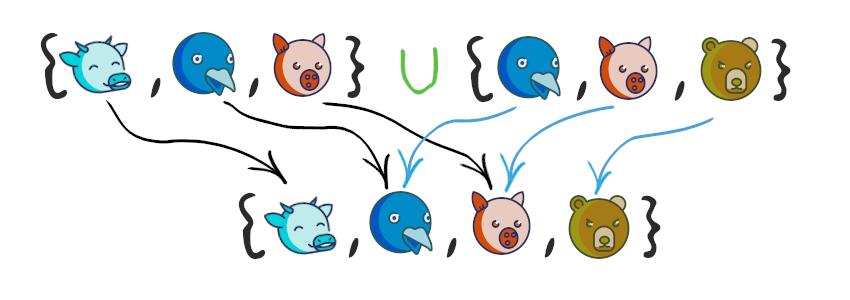
\includegraphics[width=0.35\textwidth]{set4.png}
\end{center}

Операции над множествами удобно изображать на \indef{диаграммах Эйлера-Венна:}

\begin{center}
    \begin{tikzpicture}
    % Set A
    \node [circle,
        fill=blue,
        opacity=1,
        minimum size =3cm,
        label={135:$A$}] (A) at (0,0){};
     
    % Set B
    \node [circle,
        fill=blue,
        opacity=1,
        minimum size =3cm,
        label={45:$B$}] (B) at (1.8,0){};
     
    % Circles outline
    \draw[white,thick] (0,0) circle(1.5cm);
    \draw[white,thick] (1.8,0) circle(1.5cm);
     
    % Union text label
    \node[blue!90!black] at (0.9,1.8) {$A \cup B$};
     
    \end{tikzpicture}
\end{center}

\begin{mydef} 
\indef{Пересечением} множеств $A$ и $B$ называется такое множество, которое состоит из тех и только тех  элементов, которые принадлежат и $A$, и $B$.
  
  \[A \cap B = \{x: x \in A \text{ и } x \in B \} \]
\end{mydef} 

\begin{center}
    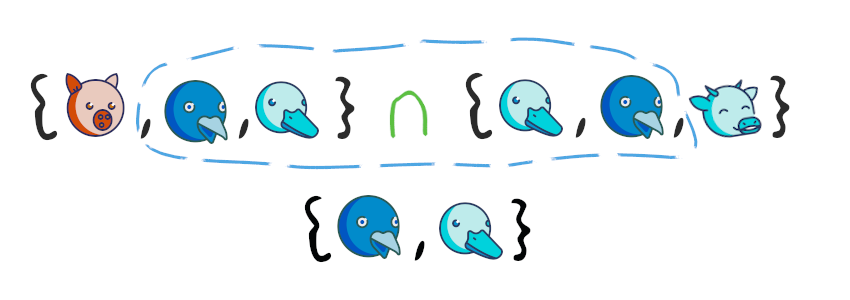
\includegraphics[width=0.35\textwidth]{set5.png}
\end{center}

Иногда бывает так, что пересечение множеств оказывается пустым.

\begin{center}
    
\includegraphics[width=0.35\textwidth]{set6.png}
\end{center}

Пересечение множеств можно изобразить на диаграме Эйлера-Вена:

\begin{center}
    \begin{tikzpicture}[thick,
            set/.style = {circle,
            minimum size = 3cm,
            fill=blue!50}]
        % Set A
        \node[set,label={135:$A$}] (A) at (0,0) {};
         
        % Set B
        \node[set,label={45:$B$}] (B) at (1.8,0) {};
         
        % Intersection
        \begin{scope}
            \clip (0,0) circle(1.5cm);
            \clip (1.8,0) circle(1.5cm);
            \fill[blue](0,0) circle(1.5cm);
        \end{scope}
         
        % Circles outline
        \draw (0,0) circle(1.5cm);
        \draw (1.8,0) circle(1.5cm);
         
        % Set intersection label
        \node[white] at (0.9,0) {$A\cap B$};
    \end{tikzpicture}
\end{center}

\begin{mydef} 
    \indef{Разностью} множеств $A$ и $B$ называется такое множество, которое состоит из тех и только тех элементов множества $A$, которые не содержатся в $B$
  
  \[A \backslash B = \{x: x \in A \text{ и }  x \notin B\}.\]
\end{mydef} 

\begin{center}
    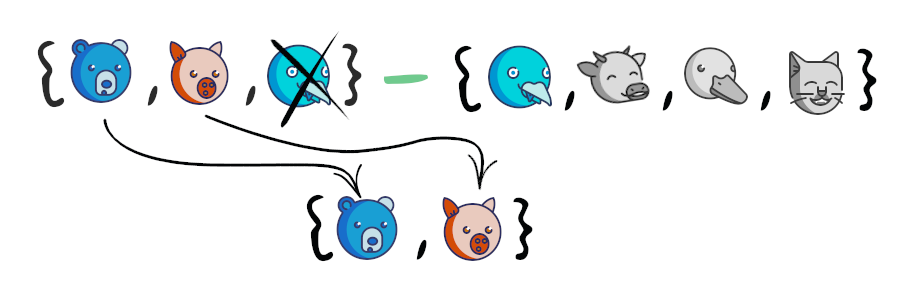
\includegraphics[width=0.35\textwidth]{set7.png}
\end{center}

\begin{center}
    \begin{tikzpicture}[thick,
        set/.style = { circle, minimum size = 3cm}]
        % Set A
        \node[set,fill=blue,label={135:$A$}] (A) at (0,0) {};
         
        % Set B
        \node[set,fill=white,label={45:$B$}] (B) at (0:2) {};
         
        % Circles outline
        \draw (0,0) circle(1.5cm);
        \draw (2,0) circle(1.5cm);
         
        % Difference text label
        \node[left,white] at (A.center){$A \backslash B$};
    \end{tikzpicture}
\end{center}


\begin{mydef}
\indef{Симметрической разностью (кольцевой суммой)} называются множество, которое включает в себя все те элементы, которые принадлежат только одному из множеств

\[A \Delta B = (A \backslash B) \cup (B \backslash A),\]

либо 

\[A \Delta B =(A \cup B) \backslash (B \cap A).\]
\end{mydef}

\begin{center}
    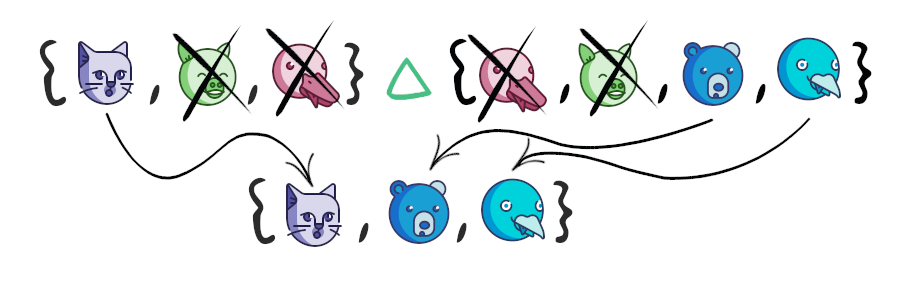
\includegraphics[width=0.35\textwidth]{set8.png}
\end{center}


\begin{mydef}
\indef{Дополнением} множества $A$ называют множества всех элементов универсального множества $U$, не входящих во множество $A$

\[\bar{A} = \{x: x \notin A \text{ и } x \in U \}.\]
\end{mydef}


\section{Свойства операций над множествами} 

Как и у любых операций, у операций над множествами есть куча свойств. Давайте приведём тут большой список хороших свойств и немного на него посмотрим. 

\begin{enumerate}
    \item От перестановки мест слагаемых сумма не меняется (коммутативность)
    \begin{equation}
        \begin{aligned}
            A \cup B = B \cup A \\
            A \cap B = B \cap A
        \end{aligned}
    \end{equation}
    
    \item Можно расставлять и раскрывать скобки (ассоциативность) 
    \begin{equation}
        \begin{aligned}
           (A \cup B) \cup C = A \cup (B \cup C) \\
           (A \cap B) \cap C = A \cap (B \cap C) \\
        \end{aligned}
    \end{equation}
    
    \item Дистрибутивность 
    \begin{equation}
        \begin{aligned}
           (A \cup B) \cap C = (A \cap C) \cup (B \cap C) \\
           (A \cap B) \cup C = (A \cup C) \cap (B \cup C) \\
        \end{aligned}
    \end{equation}    
    
    \item Законы двойственности(де Моргана):
    \begin{equation}
        \begin{aligned}
            \overline{\overline{A} \cup \overline{B}} = \overline{A} \cap \overline{B}  \\
            \overline{\overline{A} \cap \overline{B}} = \overline{A} \cup \overline{B} 
        \end{aligned}
    \end{equation}       

    \item Законы идемпотентности:
    \begin{equation}
        \begin{aligned}
            A \cup A = A \\
            A \cup \varnothing = A \\
            A \cup U = U \\
            A \cap A = A \\
            A \cap \varnothing = \varnothing \\
            A \cap U = A         
        \end{aligned}
    \end{equation}    
    
    \item Законы поглощения:
    \begin{equation}
        \begin{aligned} 
            A \cup (A \cap B) = A \\
            A \cap (A \cup B) = A
        \end{aligned}
    \end{equation}
    
    \item Закон включения:
    \begin{equation}
        \begin{aligned} 
            A \subseteq B \Leftrightarrow \bar{B} \subseteq \bar{A}
        \end{aligned}
    \end{equation}
    
    \item Закон двойного дополнения:
        \[\bar{\bar{A}} = A\]
        
    \item Закон равенства:
        \[A = B \Leftrightarrow (A \subseteq B) \cap (B \subseteq A)\]
\end{enumerate}    

Можно вывести ещё много разных свойств. Не надо запоминать их наизусть. Когда они нам будут полезны на практике, мы будем их выводить. Список нужен здесь просто для знакомства.

\section{Декартово произведение множеств}

\begin{mydef}
Пусть даны множества $A$ и $B$, пара $(a, b)$, где $a \in A, b \in B$ называется \indef{упорядоченной}. 

Множество всех упорядоченных пар вида $(a, b)$ называется \indef{декартовым произведением} множеств $A$ и $B$

\[A \times B = \{(a,b) \mid a \in A, b \in B\}.\]

Отметим, что 

\[A \times B \neq B \times A.\]
\end{mydef}

\begin{mydef}
Пусть даны множества $A_1, A_2, A_3, \ldots, A_n$ \indef{Декартовым произведением} этих множеств называется множества упорядоченных наборов $(a_1, a_2, a_3, \ldots, a_n$, где $a_i \in A_i.$ В частности, если $A_1 = A_2 = \ldots = A_n$, то $A_1 \times A_2 \times \ldots \times A_n = A^n$.
\end{mydef}

У декартового произведения тоже есть куча свойств. Вот некоторые из них:

\begin{enumerate}
    \item $(A \cup B) \times C = (A \times C) \cup (B \times C)$
    \item $(A \cap B) \times C = (A \times C) \cap (B \times C)$
    \item $(A \backslash B) \times C = (A \times C) \backslash (B \times C)$
    \item $C \times  (A \backslash B) = (C \times A) \backslash (C \times B)$
\end{enumerate}

Пусть $A$ и $B$ --- конечные множества. Напомним, что \indef{мощностью} конечного множества называется число его элементов. 

\begin{myth}
Мощность декартова произведения конечного числа конечных множеств равно произведению мощностей этих множеств, то есть 

\[
|A_1 \times A_2 \times ... \times  A_n| = |A_1| \times |A_2| \times ... \times |A_n|.
\]
\end{myth}

\section{SQL-картиночки}

\begin{center}
    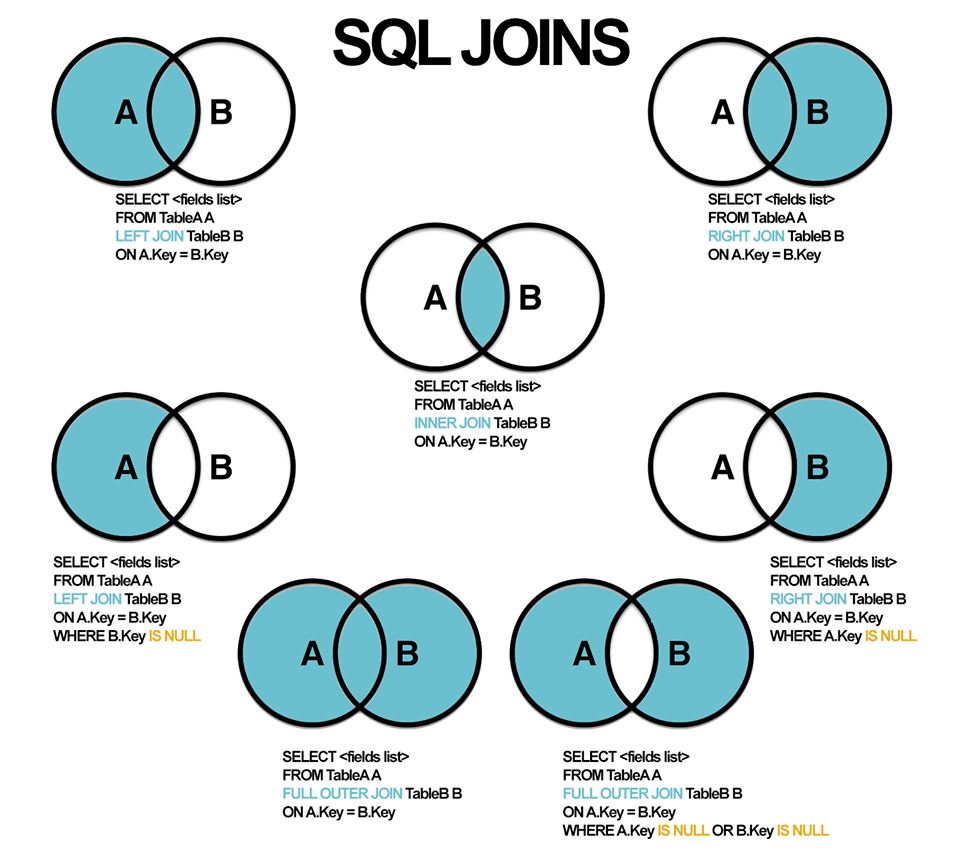
\includegraphics[width=0.85\textwidth]{sql.png}
\end{center}

Часто при написании \textbf{SQL}-запросов надо объединять таблицы по какому-то полю, индексу. В документации можно встретить диаграммы Эйлера-Вена, илюстрирующие разные типы объединения (джойнов) таблиц.

В центре картинки находится \textbf{INNER JOIN.} При нём в итоговой таблице остаются строки с ключами \textit{key}, которые были в обеих таблицах. Например, если в колонке  \textit{key} записано имя, а Ратибор есть в обеих таблицах, он попадёт и в итоговую. Если Добронрав есть только в левой или в правой таблице, он не попадёт в итоговую. Все остальные операции можно проинтерпретировать аналогичным образом.

Все основные виды \textbf{JOIN} строят декартово произведение строк по совпадающим значениям ключей. Иногда аналитики случайно пытаются поджойнить таблицы по неуникальным ключам. Например, имя Маша повторяется в таблице $A$ десять раз и в таблице $B$ двадцать раз. SQL попытается сделать декартово произведение каждой строки с каждой и для имени Маша в итоговую таблицу запишет все возможные комбинации. То есть, $200$ строк. Если ваш \textbf{JOIN} работает очень медленно, задумайтесь о своих декартовых произведениях. 

% \section{Троичная логика}

% Давайте представи себе, что у нас в табличке есть колонка типа optional bool. Она принимает три значения: True, False и NULL. В наблюдениях бывают пропуски. С ними ничего не поделаешь. Тогда возникает вопрос: что должно получиться, если мы пытаемся найти, например

% \[
% \text{True AND NULL}?
% \]

% На этот вопрос отвечают стандарты SQL, в том числе троичная логика. 

\section{Бесконечности бывают разными}

\begin{mydef}
Множества\footnote{Все следующие разделы я взял из нашей с Борисом Демешевым попытки написать книгу \newline \url{https://github.com/bdemeshev/sc_book}} $A$ и $B$ называются \indef{равномощными}, если между элементами этих множеств существует взаимно-однозначное соответствие. Мощность множества $A$ обозначается $|A|$. Соответственно равномощность двух множеств можно записать как $|A|=|B|$.
\end{mydef}

Множества $\{1,2,3,4\}$ и $\{5,11,12,17\}$ равномощны, так как есть взаимно-однозначное соответствие:

\begin{center}
    \definecolor{qqqqff}{rgb}{0.,0.,1.}
    \definecolor{qqttcc}{rgb}{0.,0.2,0.8}
    \definecolor{qqqqcc}{rgb}{0.,0.,0.8}
    \begin{tikzpicture}[line cap=round,x=1.0cm,y=1.0cm]
        \clip(-0.7941728581796409,-2.9900066347568117) rectangle (10.560863242043467,3.5563131098557585);
        \draw [rotate around={90.:(2.,0.)},line width=1.6pt,color=qqqqcc] (2.,0.) ellipse (2.7489679841754673cm and 1.8859546595880108cm);
        \draw [rotate around={90.:(8.,0.)},line width=1.6pt,color=qqttcc] (8.,0.) ellipse (2.7489679841754686cm and 1.885954659588012cm);
        \draw [->] (2.,1.5) -- (8.,1.5);
        \draw [->,line width=0.4pt] (8.,1.5) -- (2.,1.5);
        \draw [->,line width=0.4pt] (2.,0.5) -- (8.,0.5);
        \draw [->,line width=0.4pt] (8.,0.5) -- (2.,0.5);
        \draw [->,line width=0.4pt] (2.,-0.5) -- (8.,-0.5);
        \draw [->,line width=0.4pt] (8.,-0.5) -- (2.,-0.5);
        \draw [->,line width=0.4pt] (2.,-1.5) -- (8.,-1.5);
        \draw [->,line width=0.4pt] (8.,-1.5) -- (2.,-1.5);
        \draw (1.5,1.9803472454119917) node[anchor=north west] {$1$};
        \draw (1.5,0.9835825106355921) node[anchor=north west] {$2$};
        \draw (1.5,-0.04012181156719667) node[anchor=north west] {$3$};
        \draw (1.5,-1.009946958917207) node[anchor=north west] {$4$};
        \draw (8,1.966877451698797) node[anchor=north west] {$5$};
        \draw (8,0.9701127169223975) node[anchor=north west] {$11$};
        \draw (8,-0.02665201785400208) node[anchor=north west] {$12$};
        \draw (8,-1.0503563400567908) node[anchor=north west] {$17$};
        \begin{scriptsize}
        \draw [fill=qqqqff] (2.,1.5) circle (2.0pt);
        \draw [fill=qqqqff] (2.,0.5) circle (2.0pt);
        \draw [fill=qqqqff] (2.,-0.5) circle (2.0pt);
        \draw [fill=qqqqff] (2.,-1.5) circle (2.0pt);
        \draw [fill=qqqqff] (8.,1.5) circle (2.0pt);
        \draw [fill=qqqqff] (8.,0.5) circle (2.0pt);
        \draw [fill=qqqqff] (8.,-0.5) circle (2.0pt);
        \draw [fill=qqqqff] (8.,-1.5) circle (2.0pt);
        \end{scriptsize}
    \end{tikzpicture}
\end{center}

% \begin{blits}
% Какую мощность имеет множество $\{1,2,3,4\}$?
% % \begin{blitssol}
% % Мощность множества $\{1,2,3,4\}$ равна четырем.
% % \end{blitssol}
% \end{blits}

Множество $\NN$ натуральных чисел и множество чётных натуральных чисел равномощны в~силу соответствия:

\begin{center}
\definecolor{qqqqff}{rgb}{0.,0.,1.}
\definecolor{qqttcc}{rgb}{0.,0.2,0.8}
\definecolor{qqqqcc}{rgb}{0.,0.,0.8}
    \begin{tikzpicture}[line cap=round,x=1.0cm,y=1.0cm]
        \clip(-0.6996463962165264,-3.012299263838123) rectangle (10.632299575720438,2.9415664035795372);
        \draw [rotate around={90.:(2.,0.)},line width=1.6pt,color=qqqqcc] (2.,0.) ellipse (2.7489679841754673cm and 1.8859546595880108cm);
        \draw [rotate around={90.:(8.,0.)},line width=1.6pt,color=qqttcc] (8.,0.) ellipse (2.7489679841754686cm and 1.885954659588012cm);
        \draw [->] (2.,2.) -- (8.,2.);
        \draw [->,line width=0.4pt] (8.,2.) -- (2.,2.);
        \draw [->,line width=0.4pt] (2.,1.2) -- (8.,1.2);
        \draw [->,line width=0.4pt] (8.,1.2) -- (2.,1.2);
        \draw [->,line width=0.4pt] (2.,0.2) -- (8.,0.2);
        \draw [->,line width=0.4pt] (8.,0.2) -- (2.,0.2);
        \draw [->,line width=0.4pt] (2.,-0.8) -- (8.,-0.8);
        \draw [->,line width=0.4pt] (8.,-0.8) -- (2.,-0.8);
        \draw (1.5,2.4392855550936856) node[anchor=north west] {$1$};
        \draw (1.5,1.6429866489575786) node[anchor=north west] {$2$};
        \draw (1.5,0.6261741995837806) node[anchor=north west] {$3$};
        \draw (1.5,-0.36613674498582954) node[anchor=north west] {$4$};
        \draw (8,2.4637870598978733) node[anchor=north west] {$2$};
        \draw (8,1.6307358965554846) node[anchor=north west] {$4$};
        \draw (8,0.6384249519858746) node[anchor=north west] {$6$};
        \draw (8,-0.3538859925837356) node[anchor=north west] {$8$};
        \draw [->,line width=0.4pt] (2.,-2.) -- (8.,-2.);
        \draw [->,line width=0.4pt] (8.,-2.) -- (2.,-2.);
        \draw (1.5,-1.5667104803910368) node[anchor=north west] {$n$};
        \draw (8.,-1.5422089755868489) node[anchor=north west] {$2n$};
        \draw (7.7,-1.19) node[anchor=north west] {$\dots$};
        \draw (7.7,-2.22) node[anchor=north west] {$\dots$};
        \draw (1.7,-1.19) node[anchor=north west] {$\dots$};
        \draw (1.7,-2.22) node[anchor=north west] {$\dots$};
        \begin{scriptsize}
        \draw [fill=qqqqff] (2.,2.) circle (2.0pt);
        \draw [fill=qqqqff] (2.,1.2) circle (2.0pt);
        \draw [fill=qqqqff] (2.,0.2) circle (2.0pt);
        \draw [fill=qqqqff] (2.,-0.8) circle (2.0pt);
        \draw [fill=qqqqff] (8.,2.) circle (2.0pt);
        \draw [fill=qqqqff] (8.,1.2) circle (2.0pt);
        \draw [fill=qqqqff] (8.,0.2) circle (2.0pt);
        \draw [fill=qqqqff] (8.,-0.8) circle (2.0pt);
        \draw [fill=qqqqff] (2.,-2.) circle (2.0pt);
        \draw [fill=qqqqff] (8.,-2.) circle (2.0pt);
        \end{scriptsize}
    \end{tikzpicture}
\end{center}

Заметим, что в~определении требуется только существование взаимно-однозначного соответствия. Это не~противоречит тому, что могут существовать другие, не~взаимно-однозначные соответствия. Например, можно добиться и того, что среди натуральных чисел останутся «лишние»:

\begin{center}
    \definecolor{qqqqff}{rgb}{0.,0.,1.}
    \definecolor{qqttcc}{rgb}{0.,0.2,0.8}
    \definecolor{qqqqcc}{rgb}{0.,0.,0.8}
    \begin{tikzpicture}[line cap=round,x=1.0cm,y=1.0cm]
        \clip(-0.7666616663680121,-3.3866122567793884) rectangle (11.148382983444685,3.1344594772397105);
        \draw [rotate around={90.:(2.,0.)},line width=1.6pt,color=qqqqcc] (2.,0.) ellipse (2.7489679841754673cm and 1.8859546595880108cm);
        \draw [rotate around={90.:(8.,0.)},line width=1.6pt,color=qqttcc] (8.,0.) ellipse (2.7489679841754686cm and 1.885954659588012cm);
        \draw [->] (2.,2.) -- (7.8,2.);
        \draw [->,line width=0.4pt] (7.8,2.) -- (2.,2.);
        \draw [->,line width=0.4pt] (2.,1.2) -- (7.8,1.2);
        \draw [->,line width=0.4pt] (7.8,1.2) -- (2.,1.2);
        \draw [->,line width=0.4pt] (2.,0.2) -- (7.8,0.2);
        \draw [->,line width=0.4pt] (7.8,0.2) -- (2.,0.2);
        \draw [->,line width=0.4pt] (2.,-0.8) -- (7.8,-0.8);
        \draw [->,line width=0.4pt] (7.8,-0.8) -- (2.,-0.8);
        \draw (1.5,2.463567323534042) node[anchor=north west] {$1$};
        \draw (1.5,1.6584967390872398) node[anchor=north west] {$2$};
        \draw (1.5,0.6387406654546235) node[anchor=north west] {$3$};
        \draw (1.5,-0.35417972202976605) node[anchor=north west] {$4$};
        \draw (7.8,2.530656538904609) node[anchor=north west] {$???$};
        \draw (7.8,1.7121681113836933) node[anchor=north west] {$2$};
        \draw (7.8,0.7326655669734171) node[anchor=north west] {$4$};
        \draw (7.8,-0.2870905066591992) node[anchor=north west] {$6$};
        \draw [->,line width=0.4pt] (2.,-2.) -- (7.8,-2.);
        \draw [->,line width=0.4pt] (7.8,-2.) -- (2.,-2.);
        \draw (7.5,-1.19) node[anchor=north west] {$\dots$};
        \draw (1.5814608716018326,-1.5483677556258562) node[anchor=north west] {$n$};
        \draw (7.8,-1.4946963833294027) node[anchor=north west] {\small{$2n-2$}};
        \draw (7.5,-2.22) node[anchor=north west] {$\dots$};
        \draw (1.7,-1.19) node[anchor=north west] {$\dots$};
        \draw (1.7,-2.22) node[anchor=north west] {$\dots$};
        \begin{scriptsize}
        \draw [fill=qqqqff] (2.,2.) circle (2.0pt);
        \draw [fill=qqqqff] (2.,1.2) circle (2.0pt);
        \draw [fill=qqqqff] (2.,0.2) circle (2.0pt);
        \draw [fill=qqqqff] (2.,-0.8) circle (2.0pt);
        \draw [fill=qqqqff] (7.8,2.) circle (2.0pt);
        \draw [fill=qqqqff] (7.8,1.2) circle (2.0pt);
        \draw [fill=qqqqff] (7.8,0.2) circle (2.0pt);
        \draw [fill=qqqqff] (7.8,-0.8) circle (2.0pt);
        \draw [fill=qqqqff] (2.,-2.) circle (2.0pt);
        \draw [fill=qqqqff] (7.8,-2.) circle (2.0pt);
        \end{scriptsize}
    \end{tikzpicture}
\end{center}

Можно добиться того, что среди чётных останутся «лишние», а~именно:

\begin{center}
    \definecolor{qqqqff}{rgb}{0.,0.,1.}
    \definecolor{qqttcc}{rgb}{0.,0.2,0.8}
    \definecolor{qqqqcc}{rgb}{0.,0.,0.8}
    \begin{tikzpicture}[line cap=round,x=1.0cm,y=1.0cm]
        \clip(-0.7666616663680121,-3.3866122567793884) rectangle (11.148382983444685,3.1344594772397105);
        \draw [rotate around={90.:(2.,0.)},line width=1.6pt,color=qqqqcc] (2.,0.) ellipse (2.7489679841754673cm and 1.8859546595880108cm);
        \draw [rotate around={90.:(8.,0.)},line width=1.6pt,color=qqttcc] (8.,0.) ellipse (2.7489679841754686cm and 1.885954659588012cm);
        \draw [->] (2.,2.) -- (7.8,2.);
        \draw [->,line width=0.4pt] (7.8,2.) -- (2.,2.);
        \draw [->,line width=0.4pt] (2.,1.2) -- (7.8,1.2);
        \draw [->,line width=0.4pt] (7.8,1.2) -- (2.,1.2);
        \draw [->,line width=0.4pt] (2.,0.2) -- (7.8,0.2);
        \draw [->,line width=0.4pt] (7.8,0.2) -- (2.,0.2);
        \draw [->,line width=0.4pt] (2.,-0.8) -- (7.8,-0.8);
        \draw [->,line width=0.4pt] (7.8,-0.8) -- (2.,-0.8);
        \draw (1.5,2.463567323534042) node[anchor=north west] {$???$};
        \draw (1.5,1.6584967390872398) node[anchor=north west] {$1$};
        \draw (1.5,0.6387406654546235) node[anchor=north west] {$2$};
        \draw (1.5,-0.35417972202976605) node[anchor=north west] {$3$};
        \draw (7.8,2.530656538904609) node[anchor=north west] {$2$};
        \draw (7.8,1.7121681113836933) node[anchor=north west] {$4$};
        \draw (7.8,0.7326655669734171) node[anchor=north west] {$6$};
        \draw (7.8,-0.2870905066591992) node[anchor=north west] {$8$};
        \draw [->,line width=0.4pt] (2.,-2.) -- (7.8,-2.);
        \draw [->,line width=0.4pt] (7.8,-2.) -- (2.,-2.);
        \draw (7.5,-1.19) node[anchor=north west] {$\dots$};
        \draw (1.5814608716018326,-1.5483677556258562) node[anchor=north west] {$n$};
        \draw (7.8,-1.4946963833294027) node[anchor=north west] {\small{$2n+2$}};
        \draw (7.5,-2.22) node[anchor=north west] {$\dots$};
        \draw (1.7,-1.19) node[anchor=north west] {$\dots$};
        \draw (1.7,-2.22) node[anchor=north west] {$\dots$};
        \begin{scriptsize}
        \draw [fill=qqqqff] (2.,2.) circle (2.0pt);
        \draw [fill=qqqqff] (2.,1.2) circle (2.0pt);
        \draw [fill=qqqqff] (2.,0.2) circle (2.0pt);
        \draw [fill=qqqqff] (2.,-0.8) circle (2.0pt);
        \draw [fill=qqqqff] (7.8,2.) circle (2.0pt);
        \draw [fill=qqqqff] (7.8,1.2) circle (2.0pt);
        \draw [fill=qqqqff] (7.8,0.2) circle (2.0pt);
        \draw [fill=qqqqff] (7.8,-0.8) circle (2.0pt);
        \draw [fill=qqqqff] (2.,-2.) circle (2.0pt);
        \draw [fill=qqqqff] (7.8,-2.) circle (2.0pt);
        \end{scriptsize}
    \end{tikzpicture}
\end{center}

Множества $\{1,2,3,4\}$ и множество $\NN$ неравномощны. При любой попытке построить взаимно-однозначное соответствие среди натуральных чисел останутся «лишние». Возникает естественный вопрос, все~ли бесконечные множества равномощны?

Пусть $S$ множество всех бесконечных вправо последовательностей из $0$ и $1.$ Например, одним из~элементов $S$ является последовательность $1010101010\ldots$

\newpage

\begin{myth} 
Множество $S$ бесконечно, но не~равномощно множеству $\NN$.
\end{myth}

\begin{proof} Допустим противоположное, что $S$ и $\NN$ равномощны. Тогда существует взаимно-однозначное соответствие между натуральными числами и последовательностями. К~примеру оно могло~бы выглядеть так:

\begin{center}
    \definecolor{qqqqff}{rgb}{0.,0.,1.}
    \definecolor{qqttcc}{rgb}{0.,0.2,0.8}
    \definecolor{qqqqcc}{rgb}{0.,0.,0.8}
    \begin{tikzpicture}[line cap=round,x=1cm,y=1cm]
        \clip(-0.7941728581796409,-2.9900066347568117) rectangle (10.560863242043467,3.5563131098557585);
        \draw [rotate around={90.:(2.,0.)},line width=1.6pt,color=qqqqcc] (2.,0.) ellipse (2.7489679841754673cm and 1.8859546595880108cm);
        \draw [rotate around={90.:(8,0.)},line width=1.6pt,color=qqttcc] (8,0.) ellipse (2.7489679841754686cm and 1.885954659588012cm);
        \draw [->] (2.,1.5) -- (7.5,1.5);
        \draw [->,line width=0.4pt] (7.5,1.5) -- (2.,1.5);
        \draw [->,line width=0.4pt] (2.,0.5) -- (7.5,0.5);
        \draw [->,line width=0.4pt] (7.5,0.5) -- (2.,0.5);
        \draw [->,line width=0.4pt] (2.,-0.5) -- (7.5,-0.5);
        \draw [->,line width=0.4pt] (7.5,-0.5) -- (2.,-0.5);
        \draw [->,line width=0.4pt] (2.,-1.5) -- (7.5,-1.5);
        \draw [->,line width=0.4pt] (7.5,-1.5) -- (2.,-1.5);
        \draw (1.5,1.9803472454119917) node[anchor=north west] {$1$};
        \draw (1.5,0.9835825106355921) node[anchor=north west] {$2$};
        \draw (1.5,-0.04012181156719667) node[anchor=north west] {$3$};
        \draw (1.5,-1.009946958917207) node[anchor=north west] {$4$};
        \draw (7.5,1.966877451698797) node[anchor=north west] {\small{$00000\ldots$}};
        \draw (7.5,0.9701127169223975) node[anchor=north west] {\small{$01100\ldots$}};
        \draw (7.5,-0.02665201785400208) node[anchor=north west] {\small{$10101\ldots$}};
        \draw (7.5,-1.0503563400567908) node[anchor=north west] {\small{$10100\ldots$}};
        \draw (7.7,-1.8) node[anchor=north west] {$\dots$};
        \draw (1.7,-1.8) node[anchor=north west] {$\dots$};
        \begin{scriptsize}
        \draw [fill=qqqqff] (2.,1.5) circle (2.0pt);
        \draw [fill=qqqqff] (2.,0.5) circle (2.0pt);
        \draw [fill=qqqqff] (2.,-0.5) circle (2.0pt);
        \draw [fill=qqqqff] (2.,-1.5) circle (2.0pt);
        \draw [fill=qqqqff] (7.5,1.5) circle (2.0pt);
        \draw [fill=qqqqff] (7.5,0.5) circle (2.0pt);
        \draw [fill=qqqqff] (7.5,-0.5) circle (2.0pt);
        \draw [fill=qqqqff] (7.5,-1.5) circle (2.0pt);
        \end{scriptsize}
    \end{tikzpicture}
\end{center}

Оказывается какое~бы соответствие ни~было создано, всегда существует последовательность, которой не~сопоставлено ни~одно число!

Создадим последовательность $a$ по~следующему принципу: возьмем первую цифру из~первой последовательности, затем вторую из~второй, затем третью из~третьей и т.д.

\begin{center}
    \definecolor{qqqqff}{rgb}{0.,0.,1.}
    \definecolor{qqttcc}{rgb}{0.,0.2,0.8}
    \definecolor{qqqqcc}{rgb}{0.,0.,0.8}
        \begin{tikzpicture}[line cap=round,x=1cm,y=1cm]
        \clip(-0.7941728581796409,-2.9900066347568117) rectangle (10.560863242043467,3.5563131098557585);
        \draw [rotate around={90.:(2.,0.)},line width=1.6pt,color=qqqqcc] (2.,0.) ellipse (2.7489679841754673cm and 1.8859546595880108cm);
        \draw [rotate around={90.:(8,0.)},line width=1.6pt,color=qqttcc] (8,0.) ellipse (2.7489679841754686cm and 1.885954659588012cm);
        \draw [->] (2.,1.5) -- (7.5,1.5);
        \draw [->,line width=0.4pt] (7.5,1.5) -- (2.,1.5);
        \draw [->,line width=0.4pt] (2.,0.5) -- (7.5,0.5);
        \draw [->,line width=0.4pt] (7.5,0.5) -- (2.,0.5);
        \draw [->,line width=0.4pt] (2.,-0.5) -- (7.5,-0.5);
        \draw [->,line width=0.4pt] (7.5,-0.5) -- (2.,-0.5);
        \draw [->,line width=0.4pt] (2.,-1.5) -- (7.5,-1.5);
        \draw [->,line width=0.4pt] (7.5,-1.5) -- (2.,-1.5);
        \draw (1.5,1.9803472454119917) node[anchor=north west] {$1$};
        \draw (1.5,0.9835825106355921) node[anchor=north west] {$2$};
        \draw (1.5,-0.04012181156719667) node[anchor=north west] {$3$};
        \draw (1.5,-1.009946958917207) node[anchor=north west] {$4$};
        \draw (7.5,1.966877451698797) node[anchor=north west] {\small{$\underline{0}0000\ldots$}};
        \draw (7.5,0.9701127169223975) node[anchor=north west] {\small{$0\underline{1}100\ldots$}};
        \draw (7.5,-0.02665201785400208) node[anchor=north west] {\small{$10\underline{1}01\ldots$}};
        \draw (7.5,-1.0503563400567908) node[anchor=north west] {\small{$101\underline{0}0\ldots$}};
        \draw (7.7,-1.8) node[anchor=north west] {$\dots$};
        \draw (1.7,-1.8) node[anchor=north west] {$\dots$};
        \begin{scriptsize}
        \draw [fill=qqqqff] (2.,1.5) circle (2.0pt);
        \draw [fill=qqqqff] (2.,0.5) circle (2.0pt);
        \draw [fill=qqqqff] (2.,-0.5) circle (2.0pt);
        \draw [fill=qqqqff] (2.,-1.5) circle (2.0pt);
        \draw [fill=qqqqff] (7.5,1.5) circle (2.0pt);
        \draw [fill=qqqqff] (7.5,0.5) circle (2.0pt);
        \draw [fill=qqqqff] (7.5,-0.5) circle (2.0pt);
        \draw [fill=qqqqff] (7.5,-1.5) circle (2.0pt);
        \end{scriptsize}
    \end{tikzpicture}
\end{center}

Получаем последовательность $a=0110\ldots$ Затем построим последовательность $b$ заменив единицы на~нули, а~нули на~единицы в~последовательности $a$. В~нашем примере $b=1001\ldots $

Вне зависимости от~того, какое соответствие мы взяли, последовательность $b$ не~может идти в~нём ни~под каким номером! Она не~может идти под~номером 1, так как отличается от~первой последовательности первой цифрой. Она не~может идти под~номером 2, так как отличается от~второй последовательности второй цифрой и т.д.

Мы пришли к~противоречию, в~$S$ есть «лишняя» незанумерованная последовательность $b$. Значит $S$ и $\NN$ неравномощны.

Аналогичным способом можно построить «лишнюю» последовательность для любого другого предложенного соответствия.
\end{proof}

\begin{mydef} Мы говорим, что множество $A$ имеет мощность \indef{континуум}, \index{континуум} если оно равномощно множеству $S$ бесконечных вправо последовательностей из~0~и~1.
\end{mydef}

\begin{mydef} Множество $A$ называется \indef{счётным}, \index{счётное множество} если оно конечно или равномощно множеству $\NN$ натуральных чисел.
\end{mydef}

Будьте бдительны при~чтении других источников: некоторые авторы определяют счётные как равномощные натуральным числам, но~таких авторов меньшинство. Из данного определения следует, что \indef{несчётные} \index{несчётное множество} множества --- это бесконечные множества не~равномощные множеству $\NN$ натуральных чисел.

Оказывается, что любые бесконечные множества можно сравнивать: либо они равномощные, либо одно~из~них «больше».

\begin{myth} Если $A$ и $B$ --- два произвольных множества, то возможна одна и только одна из~трех ситуаций:
    \begin{itemize}
        \item[1)] Множества $A$ и $B$ равномощны.
        \item[2)] Множества $A$ и $B$ неравномощны, но $A$ равномощно какому-нибудь подмножеству множества $B$.
        \item[3)] Множества $A$ и $B$ неравномощны, но $B$ равномощно какому-нибудь подмножеству множества $A$.
    \end{itemize}
\end{myth}

\begin{rem} 
Доказательство можно найти в \cite{Shan:sets}. Может возникнуть вопрос, а~что тут собственно доказывать, всё же «очевидно»? Доказывать нужно два утверждения. Во-первых, что ситуации 2) и 3) не могут произойти одновременно. Во-вторых, что невозможна гипотетическая ситуация «несравнимости», когда $A$ и $B$ неравномощны, в~$A$ нет части равномощной $B$, и в~$B$ нет части равномощной $A$.
\end{rem}

Из этой теоремы следует важное следствие:

\begin{myth}
Если $A$ равномощно подмножеству $B$, то $ |A| \leq |B| $, т.е. либо мощность $A$ меньше мощности $B$, либо $A$ и $B$ равномощны.
\end{myth}

Давайте посмотрим на несколько важных примеров. \textbf{Начнём с бесконечных счётных множеств.}

\begin{itemize}
    \item Множество целых чисел $\ZZ$ --- счётное! Между множествами $\ZZ$ и $\NN$ существует взаимно-однозначное соответствие. Его можно установить, например, следующим образом. $1 \lra 0$, $2 \lra 1$, $3 \lra -1$, $4 \lra 2$ и т.д. Этот способ нумерации элементов множества $\ZZ$ показан на рисунке.

\begin{center}
    \[ \xymatrix{ & & & & & & & \\
    \dots & -3 \ar@/_3pc/[rrrrrrr] & -2 \ar@/_2pc/[rrrrr] & -1 \ar@/_1pc/[rrr] & 0 \ar@/_/[r] & 1 \ar@/_1pc/[ll] & 2 \ar@/_2pc/[llll] & 3 \ar@/_3pc/[llllll] & \dots \\
     & & & & & & & }
    \]
\end{center}

\item Множество пар натуральных чисел $\NN^{2}$ --- счётное! Все элементы множества $\NN^{2}$ можно пересчитать. Один из способов сделать это показан на рисунке.

\begin{center}
    \[ \xymatrix{
    (1,1) \ar[r] &  (1,2) \ar[ld]  &  (1,3) \ar[r]  & (1,4) \ar[ld]  & (1,5)  \ar[r] & \dots  \\
    (2,1) \ar[d] & (2,2) \ar[ru]  & (2,3) \ar[ld]  & (2,4) \ar[ur] & (2,5) &  \dots\\
    (3,1) \ar[ru] & (3,2) \ar[ld] & (3,3) \ar[ur] & (3,4) & (3,5)  & \dots \\
    (4,1) \ar[d] & (4,2) \ar[ur] & (4,3) & (4,4) & (4,5)  & \dots \\
    (5,1) \ar[ur] & (5,2) & (5,3) & (5,4) & (5,5)  & \dots \\
    \dots & \dots & \dots & \dots & \dots  }
    \]
\end{center}

Фактически было доказано, что объединение счётного количества счётных множеств счётно\footnote{Для знатоков может быть интересен тот факт, что в~этом доказательстве неявно используется аксиома выбора. Без неё можно представить $\RR$ как счётное объединение счётных множеств \cite{williams:wto}.}. А именно, множество $\NN^2$ можно разбить на счётное множество компонент: $\NN^2 = \{0\} \times \NN \cup \{1\} \times \NN \cup \{2\} \times \NN \cup \dots$ Элементы каждой компоненты можно выписать в отдельную строку, а после занумеровать.

\item Множество $\ZZ^{n}$ векторов из $n$ целых чисел  --- счётное!
Доказательство проведём по индукции. Мы уже доказали, что $\ZZ^{1}$ --- счётное множество. Теперь предположим, что $ \ZZ^{n-1} $ --- счётное. Получаем цепочку: $ |\ZZ^{n}|=| \ZZ^{n-1} \times \ZZ^{1}| =|\NN \times \NN| = |\NN| $.

\item Множество рациональных чисел $\QQ $ --- счётное! Приведём два способа занумеровать все рациональные числа.

Пусть $ f(q) $ --- это сумма модулей числителя и знаменателя дроби после сокращения, например, $ f(-2/3)=5 $. Сначала нумеруем дроби с $f(q)=1$, потом --- дроби с $ f(q)=2 $, потом --- дроби с $f(q)=3$ и т.д. В результате каждая дробь получает свой номер.

Рассмотрим другой, более наглядный способ нумерации, который изображен на рисунке ниже. В первой строке поместим все целые числа, во второй строке --- все дроби со знаменателем $2$, в третьей --- со знаменателем $3$ и т.д. После пронумеруем все элементы двигаясь по стрелочкам. Если элемент повторяется, например, мы уже пронумеровали $0$, но снова наталкиваемся на него или уже пронумеровали $1$ и наталкиваемся на $\frac{2}{2}$, то пропускаем его.

    \begin{center}
        \[ \xymatrix{
        0 \ar[r] &  1 \ar[ld]  &  -1 \ar[r]  &  2 \ar[ld]  &  -2  \ar[r] & \dots  \\
        0 \ar[d] & \dfrac{1}{2} \ar[ru]  & -\dfrac{1}{2} \ar[ld]  & \dfrac{2}{2} \ar[ur] & -\dfrac{2}{2} &  \dots\\
        0 \ar[ru] & \dfrac{1}{3} \ar[ld] & -\dfrac{1}{3} \ar[ur] & \dfrac{2}{3} & -\dfrac{2}{3}  & \dots \\
        0 \ar[d] & \dfrac{1}{4} \ar[ur] & -\dfrac{1}{4} & \dfrac{2}{4} & -\dfrac{2}{4}  & \dots \\
        0 \ar[ur] & \dfrac{1}{5} & -\dfrac{1}{5} & \dfrac{2}{5} & -\dfrac{2}{5}  & \dots \\
        \dots & \dots & \dots & \dots & \dots  }
        \]
    \end{center}
\end{itemize}

Теперь посмотрим на \textbf{множества мощности континуум.}

\begin{itemize}
\item Отрезок $[0;1]$ --- множество мощности континуум!

Покажем, что множество $[0;1]$ равномощно множеству $S$ бесконечных вправо последовательностей из $0$ и $1$. 

Любое число $x \in [0;1]$ можно записать в виде бесконечной двоичной дроби. Первый знак этой дроби равен 1 или 0 в зависимости от того, попадает ли число $x$ в левую или правую половину отрезка. Чтобы выбрать следующий знак, надо снова поделить выбранную половину пополам и посмотреть, куда попадет $x$, и т.д.

\begin{center}
    \definecolor{qqccqq}{rgb}{0.,0.8,0.}
    \definecolor{ffqqtt}{rgb}{1.,0.,0.2}
    \definecolor{sqsqsq}{rgb}{0.12549019607843137,0.12549019607843137,0.12549019607843137}
    \begin{tikzpicture}[line cap=round,x=1.0cm,y=1.0cm]
        \clip(-0.68061921052403,-0.058237915472957105) rectangle (8.967768719684198,1.804763819018458);
        \draw (0.1,1.04)-- (8.44,1.04);
        \draw (0.06458148327254054,1.0007314915011105) node[anchor=north west] {$0$};
        \draw (8.448089288483958,0.9517051300671259) node[anchor=north west] {$1$};
        \draw [color=ffqqtt](1.5255670540052906,0.99) node[anchor=north west] {$x$};
        \draw [shift={(3.94,1.04)},line width=0.4pt]  plot[domain=0.:1.5707963267948966,variable=\t]({1.*0.33*cos(\t r)+0.*0.33*sin(\t r)},{0.*0.33*cos(\t r)+1.*0.33*sin(\t r)});
        \draw [->] (3.94,1.37) -- (3.62,1.36);
        \draw [shift={(1.86,1.04)},line width=0.4pt]  plot[domain=0.:1.5707963267948961,variable=\t]({1.*0.33*cos(\t r)+0.*0.33*sin(\t r)},{0.*0.33*cos(\t r)+1.*0.33*sin(\t r)});
        \draw [shift={(1.56,1.02)},line width=0.4pt]  plot[domain=3.141592653589793:4.527041030388993,variable=\t]({1.*0.42*cos(\t r)+0.*0.42*sin(\t r)},{0.*0.42*cos(\t r)+1.*0.42*sin(\t r)});
        \draw [color=qqccqq](4.163185299153678,1.794958546731661) node[anchor=north west] {$0$};
        \draw [color=qqccqq](2.1040781189263122,1.7361269130108796) node[anchor=north west] {$0$};
        \draw [color=qqccqq](1.1627719793938023,0.5692995108820459) node[anchor=north west] {$1$};
        \draw [->] (1.865392886480613,1.3699559315657284) -- (1.6531471045338928,1.3775585806617356);
        \draw [->] (1.451478807241807,0.6142622143276042) -- (1.6814631100861652,0.6130264307503793);
        \draw (0.8,1) node[anchor=north west] {$\frac{1}{8}$};
        \draw (2,1) node[anchor=north west] {$\frac{1}{4}$};
        \draw (4,1) node[anchor=north west] {$\frac{1}{2}$};
        \begin{scriptsize}
        \draw [fill=black] (0.1,1.04) circle (0.5pt);
        \draw [fill=black] (8.44,1.04) circle (0.5pt);
        \draw [fill=sqsqsq] (1.68,1.04) circle (1.0pt);
        \draw [fill=black] (4.27,1.04) circle (0.5pt);
        \draw [fill=black] (2.185,1.04) circle (0.5pt);
        \draw [fill=black] (1.1425,1.04) circle (0.5pt);
        \end{scriptsize}
    \end{tikzpicture}
\end{center}

Точка $1/2$ на рисунке \ref{otrS} является серединой отрезка $[0; 1]$. Точка $x$ лежит левее $1/2$, то есть попадает в левую половину отрезка. Первый знак в элементе из $S$, который соответствует $x$ будет 0. Точка $1/4$ является серединой левой  половины отрезка $[0;1]$. Точка $x$ снова находится левее $1/4$, значит второй знак в элементе из $S$ также будет 0. Точка $1/8$ является серединой отрезка $[0; 1/4]$. Точка $x$ находится правее $1/8$, значит третий знак в элементе из $S$ будет 1. Далее посмотрим в какой части отрезка $[1/8; 1/4]$ будет лежать точка $x$ и получим четвертый знак элемента, затем пятый и так далее.

Это же соответствие можно описать в другую сторону: последовательности из нулей и единиц $x_0 x_1 x_2 \dots$ соответствует число, являющееся суммой ряда

\[ \frac{x_0}{2}+\frac{x_1}{2^2}+\frac{x_2}{2^3}+\dots \]

Например, последовательности $010100 \dots$ соответствует число

\[\frac{0}{2}+\frac{1}{2^2}+\frac{0}{2^3}+\frac{1}{2^4}+\frac{0}{2^5}+\frac{0}{2^6}+ \dots =  \frac{1}{4}+\frac{1}{16}= \frac{5}{16}.\]

Описанное соответствие пока что не совсем взаимно-однозначное: дроби вида $m/2^n$ имеют два представления. Например, число $3/8$ можно записать в виде $0011000 \dots$ и в виде $0010111 \dots$ Соответствие станет однозначным, если отбросить последовательности с бесконечным хвостом из единиц, кроме последовательности $01111 \dots$ Таких дробей счётное число и на мощность это никак не повлияет.

\begin{blits}
Какому числу соответствует последовательность $011111 \dots$?
\end{blits}

Последовательность $011111 \dots$ соответствует единице.

\[\frac{0}{2} + \frac{1}{2^2} + \frac{1}{2^3} + \frac{1}{2^4} + \frac{1}{2^5} + \ldots = \frac{1/2}{1-1/2} = 1.\]

Именно поэтому последовательность $011111 \dots$ нельзя отбросить.

\begin{blits}
Обычно в памяти компьютера числа хранятся в двоичной системе счисления.

\begin{itemize}
\item Можно ли данным способом хранить в памяти число $0.15$?
\item А правда ли что с точки зрения компьютера $0.4 - 0.3$ равно $0.1$?
\end{itemize}
\end{blits}

Если попытаться записать $0.15$ в виде последовательности из 0 и 1, мы получим периодическую бесконечную последовательность $0,1010101 \dots$, которую компьютер не сможет запомнить, так как объем памяти в нём ограничен.

Если выполнить сравнение $0.4 - 0.3 == 0.1$ в большинстве языков программирования (R, Python, Julia, C++, \ldots) то результатом будет FALSE.

\item Прямая $\RR$ --- множество мощности континуум!
Показать, что прямая $\RR$ --- множество мощности континуум можно с помощью следующей двухходовочки. 

\textbf{Ход первый:} найдем отображение, которое ставит каждому элементу числовой прямой во взаимно-однозначное соответствие элементы интервала $(0;1)$. Функция $y=\arctan x$ ставит каждому элементу $x \in (-\frac{\pi}{2};\frac{\pi}{2})$ в соответствие элемент числовой прямой $y \in \RR$.   

\begin{center}
\definecolor{ffqqqq}{rgb}{1.,0.,0.}
\definecolor{qqqqff}{rgb}{0.,0.,1.}
\begin{tikzpicture}[line cap=round,x=1.0cm,y=1.0cm]
\draw[->,color=black] (-4.255485610385398,0.) -- (4.623682062621667,0.);
\foreach \x in {}
\draw[shift={(\x,0)},color=black] (0pt,2pt) -- (0pt,-2pt) node[below] {\footnotesize $\x$};
\draw[->,color=black] (0.,-1.8541100440519962) -- (0.,2.1994230240599193);
\foreach \y in {}
\draw[shift={(0,\y)},color=black] (2pt,0pt) -- (-2pt,0pt) node[left] {\footnotesize $\y$};
\draw[color=black] (0pt,-10pt) node[right] {\footnotesize $0$};
\clip(-4.255485610385398,-1.8541100440519962) rectangle (4.623682062621667,2.1994230240599193);
\draw (-0.67,2.0) node[anchor=north west] {$\mathbf{\frac{\pi}{2}}$};
\draw (0.16,-1.1) node[anchor=north west] {$\mathbf{-\frac{\pi}{2}}$};
\draw[line width=1.2pt,color=qqqqff] (-4.255485610385398,-1.339993077797623) -- (-4.255485610385398,-1.339993077797623);
\draw[line width=1.2pt,color=qqqqff] (-4.255485610385398,-1.339993077797623) -- (-4.2332876912028805,-1.3388256696815186);
\draw[line width=1.2pt,color=qqqqff] (-4.2332876912028805,-1.3388256696815186) -- (-4.211089772020363,-1.3376466077833071);
\draw[line width=1.2pt,color=qqqqff] (-4.211089772020363,-1.3376466077833071) -- (-4.188891852837845,-1.3364557200527352);
\draw[line width=1.2pt,color=qqqqff] (-4.188891852837845,-1.3364557200527352) -- (-4.166693933655327,-1.335252831105074);
\draw[line width=1.2pt,color=qqqqff] (-4.166693933655327,-1.335252831105074) -- (-4.144496014472809,-1.334037762141752);
\draw[line width=1.2pt,color=qqqqff] (-4.144496014472809,-1.334037762141752) -- (-4.122298095290291,-1.3328103308687653);
\draw[line width=1.2pt,color=qqqqff] (-4.122298095290291,-1.3328103308687653) -- (-4.100100176107773,-1.3315703514127988);
\draw[line width=1.2pt,color=qqqqff] (-4.100100176107773,-1.3315703514127988) -- (-4.077902256925255,-1.3303176342349818);
\draw[line width=1.2pt,color=qqqqff] (-4.077902256925255,-1.3303176342349818) -- (-4.055704337742737,-1.3290519860422045);
\draw[line width=1.2pt,color=qqqqff] (-4.055704337742737,-1.3290519860422045) -- (-4.033506418560219,-1.3277732096959154);
\draw[line width=1.2pt,color=qqqqff] (-4.033506418560219,-1.3277732096959154) -- (-4.0113084993777015,-1.3264811041183187);
\draw[line width=1.2pt,color=qqqqff] (-4.0113084993777015,-1.3264811041183187) -- (-3.989110580195184,-1.3251754641958906);
\draw[line width=1.2pt,color=qqqqff] (-3.989110580195184,-1.3251754641958906) -- (-3.9669126610126666,-1.3238560806801203);
\draw[line width=1.2pt,color=qqqqff] (-3.9669126610126666,-1.3238560806801203) -- (-3.944714741830149,-1.3225227400853947);
\draw[line width=1.2pt,color=qqqqff] (-3.944714741830149,-1.3225227400853947) -- (-3.9225168226476317,-1.321175224583926);
\draw[line width=1.2pt,color=qqqqff] (-3.9225168226476317,-1.321175224583926) -- (-3.9003189034651142,-1.3198133118976276);
\draw[line width=1.2pt,color=qqqqff] (-3.9003189034651142,-1.3198133118976276) -- (-3.8781209842825968,-1.3184367751868422);
\draw[line width=1.2pt,color=qqqqff] (-3.8781209842825968,-1.3184367751868422) -- (-3.8559230651000793,-1.31704538293581);
\draw[line width=1.2pt,color=qqqqff] (-3.8559230651000793,-1.31704538293581) -- (-3.833725145917562,-1.3156388988347771);
\draw[line width=1.2pt,color=qqqqff] (-3.833725145917562,-1.3156388988347771) -- (-3.8115272267350444,-1.3142170816586285);
\draw[line width=1.2pt,color=qqqqff] (-3.8115272267350444,-1.3142170816586285) -- (-3.789329307552527,-1.312779685141931);
\draw[line width=1.2pt,color=qqqqff] (-3.789329307552527,-1.312779685141931) -- (-3.7671313883700095,-1.3113264578502664);
\draw[line width=1.2pt,color=qqqqff] (-3.7671313883700095,-1.3113264578502664) -- (-3.744933469187492,-1.3098571430477308);
\draw[line width=1.2pt,color=qqqqff] (-3.744933469187492,-1.3098571430477308) -- (-3.7227355500049746,-1.308371478560471);
\draw[line width=1.2pt,color=qqqqff] (-3.7227355500049746,-1.308371478560471) -- (-3.700537630822457,-1.3068691966361252);
\draw[line width=1.2pt,color=qqqqff] (-3.700537630822457,-1.3068691966361252) -- (-3.6783397116399397,-1.3053500237990299);
\draw[line width=1.2pt,color=qqqqff] (-3.6783397116399397,-1.3053500237990299) -- (-3.656141792457422,-1.3038136807010483);
\draw[line width=1.2pt,color=qqqqff] (-3.656141792457422,-1.3038136807010483) -- (-3.6339438732749048,-1.302259881967873);
\draw[line width=1.2pt,color=qqqqff] (-3.6339438732749048,-1.302259881967873) -- (-3.6117459540923873,-1.3006883360406478);
\draw[line width=1.2pt,color=qqqqff] (-3.6117459540923873,-1.3006883360406478) -- (-3.58954803490987,-1.2990987450127518);
\draw[line width=1.2pt,color=qqqqff] (-3.58954803490987,-1.2990987450127518) -- (-3.5673501157273524,-1.2974908044615734);
\draw[line width=1.2pt,color=qqqqff] (-3.5673501157273524,-1.2974908044615734) -- (-3.545152196544835,-1.2958642032751129);
\draw[line width=1.2pt,color=qqqqff] (-3.545152196544835,-1.2958642032751129) -- (-3.5229542773623175,-1.2942186234732236);
\draw[line width=1.2pt,color=qqqqff] (-3.5229542773623175,-1.2942186234732236) -- (-3.5007563581798,-1.2925537400233176);
\draw[line width=1.2pt,color=qqqqff] (-3.5007563581798,-1.2925537400233176) -- (-3.4785584389972826,-1.2908692206503358);
\draw[line width=1.2pt,color=qqqqff] (-3.4785584389972826,-1.2908692206503358) -- (-3.456360519814765,-1.2891647256407923);
\draw[line width=1.2pt,color=qqqqff] (-3.456360519814765,-1.2891647256407923) -- (-3.4341626006322477,-1.2874399076406773);
\draw[line width=1.2pt,color=qqqqff] (-3.4341626006322477,-1.2874399076406773) -- (-3.41196468144973,-1.2856944114470141);
\draw[line width=1.2pt,color=qqqqff] (-3.41196468144973,-1.2856944114470141) -- (-3.3897667622672127,-1.2839278737928435);
\draw[line width=1.2pt,color=qqqqff] (-3.3897667622672127,-1.2839278737928435) -- (-3.3675688430846953,-1.2821399231254058);
\draw[line width=1.2pt,color=qqqqff] (-3.3675688430846953,-1.2821399231254058) -- (-3.345370923902178,-1.2803301793772854);
\draw[line width=1.2pt,color=qqqqff] (-3.345370923902178,-1.2803301793772854) -- (-3.3231730047196604,-1.2784982537302674);
\draw[line width=1.2pt,color=qqqqff] (-3.3231730047196604,-1.2784982537302674) -- (-3.300975085537143,-1.2766437483716522);
\draw[line width=1.2pt,color=qqqqff] (-3.300975085537143,-1.2766437483716522) -- (-3.2787771663546255,-1.2747662562427615);
\draw[line width=1.2pt,color=qqqqff] (-3.2787771663546255,-1.2747662562427615) -- (-3.256579247172108,-1.2728653607793605);
\draw[line width=1.2pt,color=qqqqff] (-3.256579247172108,-1.2728653607793605) -- (-3.2343813279895905,-1.2709406356437098);
\draw[line width=1.2pt,color=qqqqff] (-3.2343813279895905,-1.2709406356437098) -- (-3.212183408807073,-1.2689916444479534);
\draw[line width=1.2pt,color=qqqqff] (-3.212183408807073,-1.2689916444479534) -- (-3.1899854896245556,-1.2670179404685302);
\draw[line width=1.2pt,color=qqqqff] (-3.1899854896245556,-1.2670179404685302) -- (-3.167787570442038,-1.2650190663512988);
\draw[line width=1.2pt,color=qqqqff] (-3.167787570442038,-1.2650190663512988) -- (-3.1455896512595207,-1.2629945538070362);
\draw[line width=1.2pt,color=qqqqff] (-3.1455896512595207,-1.2629945538070362) -- (-3.1233917320770033,-1.2609439232969772);
\draw[line width=1.2pt,color=qqqqff] (-3.1233917320770033,-1.2609439232969772) -- (-3.101193812894486,-1.2588666837080336);
\draw[line width=1.2pt,color=qqqqff] (-3.101193812894486,-1.2588666837080336) -- (-3.0789958937119684,-1.256762332017329);
\draw[line width=1.2pt,color=qqqqff] (-3.0789958937119684,-1.256762332017329) -- (-3.056797974529451,-1.2546303529456666);
\draw[line width=1.2pt,color=qqqqff] (-3.056797974529451,-1.2546303529456666) -- (-3.0346000553469334,-1.2524702185995404);
\draw[line width=1.2pt,color=qqqqff] (-3.0346000553469334,-1.2524702185995404) -- (-3.012402136164416,-1.2502813881012735);
\draw[line width=1.2pt,color=qqqqff] (-3.012402136164416,-1.2502813881012735) -- (-2.9902042169818985,-1.2480633072068683);
\draw[line width=1.2pt,color=qqqqff] (-2.9902042169818985,-1.2480633072068683) -- (-2.968006297799381,-1.2458154079111279);
\draw[line width=1.2pt,color=qqqqff] (-2.968006297799381,-1.2458154079111279) -- (-2.9458083786168636,-1.2435371080395932);
\draw[line width=1.2pt,color=qqqqff] (-2.9458083786168636,-1.2435371080395932) -- (-2.923610459434346,-1.2412278108268322);
\draw[line width=1.2pt,color=qqqqff] (-2.923610459434346,-1.2412278108268322) -- (-2.9014125402518287,-1.2388869044805921);
\draw[line width=1.2pt,color=qqqqff] (-2.9014125402518287,-1.2388869044805921) -- (-2.8792146210693113,-1.236513761731313);
\draw[line width=1.2pt,color=qqqqff] (-2.8792146210693113,-1.236513761731313) -- (-2.857016701886794,-1.2341077393664897);
\draw[line width=1.2pt,color=qqqqff] (-2.857016701886794,-1.2341077393664897) -- (-2.8348187827042763,-1.231668177749338);
\draw[line width=1.2pt,color=qqqqff] (-2.8348187827042763,-1.231668177749338) -- (-2.812620863521759,-1.2291944003212194);
\draw[line width=1.2pt,color=qqqqff] (-2.812620863521759,-1.2291944003212194) -- (-2.7904229443392414,-1.2266857130872482);
\draw[line width=1.2pt,color=qqqqff] (-2.7904229443392414,-1.2266857130872482) -- (-2.768225025156724,-1.2241414040844942);
\draw[line width=1.2pt,color=qqqqff] (-2.768225025156724,-1.2241414040844942) -- (-2.7460271059742065,-1.2215607428321698);
\draw[line width=1.2pt,color=qqqqff] (-2.7460271059742065,-1.2215607428321698) -- (-2.723829186791689,-1.2189429797631794);
\draw[line width=1.2pt,color=qqqqff] (-2.723829186791689,-1.2189429797631794) -- (-2.7016312676091716,-1.2162873456363812);
\draw[line width=1.2pt,color=qqqqff] (-2.7016312676091716,-1.2162873456363812) -- (-2.679433348426654,-1.2135930509288977);
\draw[line width=1.2pt,color=qqqqff] (-2.679433348426654,-1.2135930509288977) -- (-2.6572354292441367,-1.210859285207793);
\draw[line width=1.2pt,color=qqqqff] (-2.6572354292441367,-1.210859285207793) -- (-2.6350375100616192,-1.208085216480413);
\draw[line width=1.2pt,color=qqqqff] (-2.6350375100616192,-1.208085216480413) -- (-2.612839590879102,-1.205269990522667);
\draw[line width=1.2pt,color=qqqqff] (-2.612839590879102,-1.205269990522667) -- (-2.5906416716965843,-1.2024127301845107);
\draw[line width=1.2pt,color=qqqqff] (-2.5906416716965843,-1.2024127301845107) -- (-2.568443752514067,-1.1995125346718738);
\draw[line width=1.2pt,color=qqqqff] (-2.568443752514067,-1.1995125346718738) -- (-2.5462458333315494,-1.196568478804254);
\draw[line width=1.2pt,color=qqqqff] (-2.5462458333315494,-1.196568478804254) -- (-2.524047914149032,-1.1935796122471876);
\draw[line width=1.2pt,color=qqqqff] (-2.524047914149032,-1.1935796122471876) -- (-2.5018499949665145,-1.190544958718784);
\draw[line width=1.2pt,color=qqqqff] (-2.5018499949665145,-1.190544958718784) -- (-2.479652075783997,-1.187463515169504);
\draw[line width=1.2pt,color=qqqqff] (-2.479652075783997,-1.187463515169504) -- (-2.4574541566014796,-1.1843342509343406);
\draw[line width=1.2pt,color=qqqqff] (-2.4574541566014796,-1.1843342509343406) -- (-2.435256237418962,-1.181156106856553);
\draw[line width=1.2pt,color=qqqqff] (-2.435256237418962,-1.181156106856553) -- (-2.4130583182364447,-1.1779279943820953);
\draw[line width=1.2pt,color=qqqqff] (-2.4130583182364447,-1.1779279943820953) -- (-2.390860399053927,-1.1746487946238648);
\draw[line width=1.2pt,color=qqqqff] (-2.390860399053927,-1.1746487946238648) -- (-2.3686624798714098,-1.1713173573949025);
\draw[line width=1.2pt,color=qqqqff] (-2.3686624798714098,-1.1713173573949025) -- (-2.3464645606888923,-1.1679325002096597);
\draw[line width=1.2pt,color=qqqqff] (-2.3464645606888923,-1.1679325002096597) -- (-2.324266641506375,-1.16449300725246);
\draw[line width=1.2pt,color=qqqqff] (-2.324266641506375,-1.16449300725246) -- (-2.3020687223238574,-1.1609976283122774);
\draw[line width=1.2pt,color=qqqqff] (-2.3020687223238574,-1.1609976283122774) -- (-2.27987080314134,-1.157445077682969);
\draw[line width=1.2pt,color=qqqqff] (-2.27987080314134,-1.157445077682969) -- (-2.2576728839588225,-1.15383403302811);
\draw[line width=1.2pt,color=qqqqff] (-2.2576728839588225,-1.15383403302811) -- (-2.235474964776305,-1.1501631342095995);
\draw[line width=1.2pt,color=qqqqff] (-2.235474964776305,-1.1501631342095995) -- (-2.2132770455937876,-1.1464309820792293);
\draw[line width=1.2pt,color=qqqqff] (-2.2132770455937876,-1.1464309820792293) -- (-2.19107912641127,-1.1426361372324474);
\draw[line width=1.2pt,color=qqqqff] (-2.19107912641127,-1.1426361372324474) -- (-2.1688812072287527,-1.1387771187235816);
\draw[line width=1.2pt,color=qqqqff] (-2.1688812072287527,-1.1387771187235816) -- (-2.146683288046235,-1.1348524027418476);
\draw[line width=1.2pt,color=qqqqff] (-2.146683288046235,-1.1348524027418476) -- (-2.1244853688637177,-1.1308604212475202);
\draw[line width=1.2pt,color=qqqqff] (-2.1244853688637177,-1.1308604212475202) -- (-2.1022874496812003,-1.1267995605677292);
\draw[line width=1.2pt,color=qqqqff] (-2.1022874496812003,-1.1267995605677292) -- (-2.080089530498683,-1.1226681599514192);
\draw[line width=1.2pt,color=qqqqff] (-2.080089530498683,-1.1226681599514192) -- (-2.0578916113161654,-1.1184645100831234);
\draw[line width=1.2pt,color=qqqqff] (-2.0578916113161654,-1.1184645100831234) -- (-2.035693692133648,-1.1141868515553164);
\draw[line width=1.2pt,color=qqqqff] (-2.035693692133648,-1.1141868515553164) -- (-2.0134957729511305,-1.1098333732992471);
\draw[line width=1.2pt,color=qqqqff] (-2.0134957729511305,-1.1098333732992471) -- (-1.9912978537686128,-1.1054022109743198);
\draw[line width=1.2pt,color=qqqqff] (-1.9912978537686128,-1.1054022109743198) -- (-1.9690999345860951,-1.100891445316265);
\draw[line width=1.2pt,color=qqqqff] (-1.9690999345860951,-1.100891445316265) -- (-1.9469020154035774,-1.096299100444555);
\draw[line width=1.2pt,color=qqqqff] (-1.9469020154035774,-1.096299100444555) -- (-1.9247040962210598,-1.0916231421297569);
\draw[line width=1.2pt,color=qqqqff] (-1.9247040962210598,-1.0916231421297569) -- (-1.902506177038542,-1.0868614760217852);
\draw[line width=1.2pt,color=qqqqff] (-1.902506177038542,-1.0868614760217852) -- (-1.8803082578560244,-1.0820119458403175);
\draw[line width=1.2pt,color=qqqqff] (-1.8803082578560244,-1.0820119458403175) -- (-1.8581103386735067,-1.0770723315289878);
\draw[line width=1.2pt,color=qqqqff] (-1.8581103386735067,-1.0770723315289878) -- (-1.835912419490989,-1.0720403473753575);
\draw[line width=1.2pt,color=qqqqff] (-1.835912419490989,-1.0720403473753575) -- (-1.8137145003084714,-1.066913640099098);
\draw[line width=1.2pt,color=qqqqff] (-1.8137145003084714,-1.066913640099098) -- (-1.7915165811259537,-1.0616897869113144);
\draw[line width=1.2pt,color=qqqqff] (-1.7915165811259537,-1.0616897869113144) -- (-1.769318661943436,-1.0563662935484859);
\draw[line width=1.2pt,color=qqqqff] (-1.769318661943436,-1.0563662935484859) -- (-1.7471207427609183,-1.0509405922851052);
\draw[line width=1.2pt,color=qqqqff] (-1.7471207427609183,-1.0509405922851052) -- (-1.7249228235784007,-1.0454100399297994);
\draw[line width=1.2pt,color=qqqqff] (-1.7249228235784007,-1.0454100399297994) -- (-1.702724904395883,-1.0397719158104546);
\draw[line width=1.2pt,color=qqqqff] (-1.702724904395883,-1.0397719158104546) -- (-1.6805269852133653,-1.034023419754735);
\draw[line width=1.2pt,color=qqqqff] (-1.6805269852133653,-1.034023419754735) -- (-1.6583290660308476,-1.0281616700733103);
\draw[line width=1.2pt,color=qqqqff] (-1.6583290660308476,-1.0281616700733103) -- (-1.63613114684833,-1.0221837015541562);
\draw[line width=1.2pt,color=qqqqff] (-1.63613114684833,-1.0221837015541562) -- (-1.6139332276658123,-1.0160864634774451);
\draw[line width=1.2pt,color=qqqqff] (-1.6139332276658123,-1.0160864634774451) -- (-1.5917353084832946,-1.009866817661811);
\draw[line width=1.2pt,color=qqqqff] (-1.5917353084832946,-1.009866817661811) -- (-1.569537389300777,-1.003521536554182);
\draw[line width=1.2pt,color=qqqqff] (-1.569537389300777,-1.003521536554182) -- (-1.5473394701182592,-0.9970473013769171);
\draw[line width=1.2pt,color=qqqqff] (-1.5473394701182592,-0.9970473013769171) -- (-1.5251415509357416,-0.9904407003476805);
\draw[line width=1.2pt,color=qqqqff] (-1.5251415509357416,-0.9904407003476805) -- (-1.5029436317532239,-0.9836982269893491);
\draw[line width=1.2pt,color=qqqqff] (-1.5029436317532239,-0.9836982269893491) -- (-1.4807457125707062,-0.9768162785492855);
\draw[line width=1.2pt,color=qqqqff] (-1.4807457125707062,-0.9768162785492855) -- (-1.4585477933881885,-0.969791154549537);
\draw[line width=1.2pt,color=qqqqff] (-1.4585477933881885,-0.969791154549537) -- (-1.4363498742056708,-0.962619055491944);
\draw[line width=1.2pt,color=qqqqff] (-1.4363498742056708,-0.962619055491944) -- (-1.4141519550231532,-0.955296081744781);
\draw[line width=1.2pt,color=qqqqff] (-1.4141519550231532,-0.955296081744781) -- (-1.3919540358406355,-0.9478182326404136);
\draw[line width=1.2pt,color=qqqqff] (-1.3919540358406355,-0.9478182326404136) -- (-1.3697561166581178,-0.9401814058165519);
\draw[line width=1.2pt,color=qqqqff] (-1.3697561166581178,-0.9401814058165519) -- (-1.3475581974756001,-0.9323813968370139);
\draw[line width=1.2pt,color=qqqqff] (-1.3475581974756001,-0.9323813968370139) -- (-1.3253602782930824,-0.9244138991315101);
\draw[line width=1.2pt,color=qqqqff] (-1.3253602782930824,-0.9244138991315101) -- (-1.3031623591105648,-0.9162745042977944);
\draw[line width=1.2pt,color=qqqqff] (-1.3031623591105648,-0.9162745042977944) -- (-1.280964439928047,-0.9079587028136413);
\draw[line width=1.2pt,color=qqqqff] (-1.280964439928047,-0.9079587028136413) -- (-1.2587665207455294,-0.899461885210457);
\draw[line width=1.2pt,color=qqqqff] (-1.2587665207455294,-0.899461885210457) -- (-1.2365686015630117,-0.8907793437649546);
\draw[line width=1.2pt,color=qqqqff] (-1.2365686015630117,-0.8907793437649546) -- (-1.214370682380494,-0.8819062747701587);
\draw[line width=1.2pt,color=qqqqff] (-1.214370682380494,-0.8819062747701587) -- (-1.1921727631979764,-0.8728377814520804);
\draw[line width=1.2pt,color=qqqqff] (-1.1921727631979764,-0.8728377814520804) -- (-1.1699748440154587,-0.8635688776036512);
\draw[line width=1.2pt,color=qqqqff] (-1.1699748440154587,-0.8635688776036512) -- (-1.147776924832941,-0.8540944920129155);
\draw[line width=1.2pt,color=qqqqff] (-1.147776924832941,-0.8540944920129155) -- (-1.1255790056504233,-0.8444094737679816);
\draw[line width=1.2pt,color=qqqqff] (-1.1255790056504233,-0.8444094737679816) -- (-1.1033810864679057,-0.8345085985267726);
\draw[line width=1.2pt,color=qqqqff] (-1.1033810864679057,-0.8345085985267726) -- (-1.081183167285388,-0.8243865758451102);
\draw[line width=1.2pt,color=qqqqff] (-1.081183167285388,-0.8243865758451102) -- (-1.0589852481028703,-0.8140380576619984);
\draw[line width=1.2pt,color=qqqqff] (-1.0589852481028703,-0.8140380576619984) -- (-1.0367873289203526,-0.8034576480460499);
\draw[line width=1.2pt,color=qqqqff] (-1.0367873289203526,-0.8034576480460499) -- (-1.014589409737835,-0.7926399143116372);
\draw[line width=1.2pt,color=qqqqff] (-1.014589409737835,-0.7926399143116372) -- (-0.9923914905553173,-0.7815793996174086);
\draw[line width=1.2pt,color=qqqqff] (-0.9923914905553173,-0.7815793996174086) -- (-0.9701935713727996,-0.7702706371630579);
\draw[line width=1.2pt,color=qqqqff] (-0.9701935713727996,-0.7702706371630579) -- (-0.9479956521902819,-0.7587081661024563);
\draw[line width=1.2pt,color=qqqqff] (-0.9479956521902819,-0.7587081661024563) -- (-0.9257977330077642,-0.7468865492921682);
\draw[line width=1.2pt,color=qqqqff] (-0.9257977330077642,-0.7468865492921682) -- (-0.9035998138252466,-0.7348003929936731);
\draw[line width=1.2pt,color=qqqqff] (-0.9035998138252466,-0.7348003929936731) -- (-0.8814018946427289,-0.7224443686449614);
\draw[line width=1.2pt,color=qqqqff] (-0.8814018946427289,-0.7224443686449614) -- (-0.8592039754602112,-0.7098132368121983);
\draw[line width=1.2pt,color=qqqqff] (-0.8592039754602112,-0.7098132368121983) -- (-0.8370060562776935,-0.6969018734244171);
\draw[line width=1.2pt,color=qqqqff] (-0.8370060562776935,-0.6969018734244171) -- (-0.8148081370951759,-0.6837052983833114);
\draw[line width=1.2pt,color=qqqqff] (-0.8148081370951759,-0.6837052983833114) -- (-0.7926102179126582,-0.6702187066256439);
\draw[line width=1.2pt,color=qqqqff] (-0.7926102179126582,-0.6702187066256439) -- (-0.7704122987301405,-0.6564375016971316);
\draw[line width=1.2pt,color=qqqqff] (-0.7704122987301405,-0.6564375016971316) -- (-0.7482143795476228,-0.6423573318734072);
\draw[line width=1.2pt,color=qqqqff] (-0.7482143795476228,-0.6423573318734072) -- (-0.7260164603651051,-0.6279741288353444);
\draw[line width=1.2pt,color=qqqqff] (-0.7260164603651051,-0.6279741288353444) -- (-0.7038185411825875,-0.6132841488722423);
\draw[line width=1.2pt,color=qqqqff] (-0.7038185411825875,-0.6132841488722423) -- (-0.6816206220000698,-0.5982840165467278);
\draw[line width=1.2pt,color=qqqqff] (-0.6816206220000698,-0.5982840165467278) -- (-0.6594227028175521,-0.582970770709494);
\draw[line width=1.2pt,color=qqqqff] (-0.6594227028175521,-0.582970770709494) -- (-0.6372247836350344,-0.5673419126999802);
\draw[line width=1.2pt,color=qqqqff] (-0.6372247836350344,-0.5673419126999802) -- (-0.6150268644525168,-0.5513954565108754);
\draw[line width=1.2pt,color=qqqqff] (-0.6150268644525168,-0.5513954565108754) -- (-0.5928289452699991,-0.5351299806300777);
\draw[line width=1.2pt,color=qqqqff] (-0.5928289452699991,-0.5351299806300777) -- (-0.5706310260874814,-0.5185446812039874);
\draw[line width=1.2pt,color=qqqqff] (-0.5706310260874814,-0.5185446812039874) -- (-0.5484331069049637,-0.5016394260915022);
\draw[line width=1.2pt,color=qqqqff] (-0.5484331069049637,-0.5016394260915022) -- (-0.526235187722446,-0.4844148092999408);
\draw[line width=1.2pt,color=qqqqff] (-0.526235187722446,-0.4844148092999408) -- (-0.5040372685399284,-0.4668722052138426);
\draw[line width=1.2pt,color=qqqqff] (-0.5040372685399284,-0.4668722052138426) -- (-0.4818393493574107,-0.4490138219470344);
\draw[line width=1.2pt,color=qqqqff] (-0.4818393493574107,-0.4490138219470344) -- (-0.459641430174893,-0.4308427530698338);
\draw[line width=1.2pt,color=qqqqff] (-0.459641430174893,-0.4308427530698338) -- (-0.43744351099237533,-0.4123630268894431);
\draw[line width=1.2pt,color=qqqqff] (-0.43744351099237533,-0.4123630268894431) -- (-0.41524559180985765,-0.39357965239554205);
\draw[line width=1.2pt,color=qqqqff] (-0.41524559180985765,-0.39357965239554205) -- (-0.39304767262734,-0.37449866092815765);
\draw[line width=1.2pt,color=qqqqff] (-0.39304767262734,-0.37449866092815765) -- (-0.3708497534448223,-0.3551271425846554);
\draw[line width=1.2pt,color=qqqqff] (-0.3708497534448223,-0.3551271425846554) -- (-0.3486518342623046,-0.3354732763607945);
\draw[line width=1.2pt,color=qqqqff] (-0.3486518342623046,-0.3354732763607945) -- (-0.32645391507978694,-0.3155463530208032);
\draw[line width=1.2pt,color=qqqqff] (-0.32645391507978694,-0.3155463530208032) -- (-0.30425599589726926,-0.29535678971665624);
\draw[line width=1.2pt,color=qqqqff] (-0.30425599589726926,-0.29535678971665624) -- (-0.2820580767147516,-0.274916135429997);
\draw[line width=1.2pt,color=qqqqff] (-0.2820580767147516,-0.274916135429997) -- (-0.2598601575322339,-0.25423706639354726);
\draw[line width=1.2pt,color=qqqqff] (-0.2598601575322339,-0.25423706639354726) -- (-0.23766223834971625,-0.23333337076355634);
\draw[line width=1.2pt,color=qqqqff] (-0.23766223834971625,-0.23333337076355634) -- (-0.2154643191671986,-0.2122199219608644);
\draw[line width=1.2pt,color=qqqqff] (-0.2154643191671986,-0.2122199219608644) -- (-0.19326639998468095,-0.1909126402741829);
\draw[line width=1.2pt,color=qqqqff] (-0.19326639998468095,-0.1909126402741829) -- (-0.1710684808021633,-0.169428442522446);
\draw[line width=1.2pt,color=qqqqff] (-0.1710684808021633,-0.169428442522446) -- (-0.14887056161964565,-0.14778517979929523);
\draw[line width=1.2pt,color=qqqqff] (-0.14887056161964565,-0.14778517979929523) -- (-0.126672642437128,-0.1260015635661915);
\draw[line width=1.2pt,color=qqqqff] (-0.126672642437128,-0.1260015635661915) -- (-0.10447472325461034,-0.10409708061424336);
\draw[line width=1.2pt,color=qqqqff] (-0.10447472325461034,-0.10409708061424336) -- (-0.08227680407209267,-0.08209189767047104);
\draw[line width=1.2pt,color=qqqqff] (-0.08227680407209267,-0.08209189767047104) -- (-0.06007888488957501,-0.060006756673005486);
\draw[line width=1.2pt,color=qqqqff] (-0.06007888488957501,-0.060006756673005486) -- (-0.037880965707057346,-0.037862861972452526);
\draw[line width=1.2pt,color=qqqqff] (-0.037880965707057346,-0.037862861972452526) -- (-0.015683046524539685,-0.015681760924274472);
\draw[line width=1.2pt,color=qqqqff] (-0.015683046524539685,-0.015681760924274472) -- (0.006514872657977976,0.0065147804888498195);
\draw[line width=1.2pt,color=qqqqff] (0.006514872657977976,0.0065147804888498195) -- (0.028712791840495636,0.028704905232400907);
\draw[line width=1.2pt,color=qqqqff] (0.028712791840495636,0.028704905232400907) -- (0.0509107110230133,0.05086679413400104);
\draw[line width=1.2pt,color=qqqqff] (0.0509107110230133,0.05086679413400104) -- (0.07310863020553096,0.07297879424027495);
\draw[line width=1.2pt,color=qqqqff] (0.07310863020553096,0.07297879424027495) -- (0.09530654938804863,0.09501954473611073);
\draw[line width=1.2pt,color=qqqqff] (0.09530654938804863,0.09501954473611073) -- (0.11750446857056629,0.11696809861227091);
\draw[line width=1.2pt,color=qqqqff] (0.11750446857056629,0.11696809861227091) -- (0.13970238775308394,0.138804038382018);
\draw[line width=1.2pt,color=qqqqff] (0.13970238775308394,0.138804038382018) -- (0.1619003069356016,0.16050758430548354);
\draw[line width=1.2pt,color=qqqqff] (0.1619003069356016,0.16050758430548354) -- (0.18409822611811924,0.18205969377525502);
\draw[line width=1.2pt,color=qqqqff] (0.18409822611811924,0.18205969377525502) -- (0.2062961453006369,0.20344215074008734);
\draw[line width=1.2pt,color=qqqqff] (0.2062961453006369,0.20344215074008734) -- (0.22849406448315454,0.22463764428691538);
\draw[line width=1.2pt,color=qqqqff] (0.22849406448315454,0.22463764428691538) -- (0.2506919836656722,0.2456298357552503);
\draw[line width=1.2pt,color=qqqqff] (0.2506919836656722,0.2456298357552503) -- (0.27288990284818987,0.266403414013515);
\draw[line width=1.2pt,color=qqqqff] (0.27288990284818987,0.266403414013515) -- (0.29508782203070755,0.2869441387754269);
\draw[line width=1.2pt,color=qqqqff] (0.29508782203070755,0.2869441387754269) -- (0.3172857412132252,0.3072388720686329);
\draw[line width=1.2pt,color=qqqqff] (0.3172857412132252,0.3072388720686329) -- (0.3394836603957429,0.3272755981811376);
\draw[line width=1.2pt,color=qqqqff] (0.3394836603957429,0.3272755981811376) -- (0.3616815795782606,0.34704343259875936);
\draw[line width=1.2pt,color=qqqqff] (0.3616815795782606,0.34704343259875936) -- (0.38387949876077826,0.36653262060550396);
\draw[line width=1.2pt,color=qqqqff] (0.38387949876077826,0.36653262060550396) -- (0.40607741794329594,0.38573452634646066);
\draw[line width=1.2pt,color=qqqqff] (0.40607741794329594,0.38573452634646066) -- (0.4282753371258136,0.4046416132490754);
\draw[line width=1.2pt,color=qqqqff] (0.4282753371258136,0.4046416132490754) -- (0.4504732563083313,0.42324741676415917);
\draw[line width=1.2pt,color=qqqqff] (0.4504732563083313,0.42324741676415917) -- (0.47267117549084897,0.4415465104244873);
\draw[line width=1.2pt,color=qqqqff] (0.47267117549084897,0.4415465104244873) -- (0.49486909467336665,0.4595344662288935);
\draw[line width=1.2pt,color=qqqqff] (0.49486909467336665,0.4595344662288935) -- (0.5170670138558843,0.4772078103464926);
\draw[line width=1.2pt,color=qqqqff] (0.5170670138558843,0.4772078103464926) -- (0.539264933038402,0.49456397510255834);
\draw[line width=1.2pt,color=qqqqff] (0.539264933038402,0.49456397510255834) -- (0.5614628522209196,0.5116012481582837);
\draw[line width=1.2pt,color=qqqqff] (0.5614628522209196,0.5116012481582837) -- (0.5836607714034373,0.5283187197347752);
\draw[line width=1.2pt,color=qqqqff] (0.5836607714034373,0.5283187197347752) -- (0.605858690585955,0.5447162286606368);
\draw[line width=1.2pt,color=qqqqff] (0.605858690585955,0.5447162286606368) -- (0.6280566097684727,0.5607943079455725);
\draw[line width=1.2pt,color=qqqqff] (0.6280566097684727,0.5607943079455725) -- (0.6502545289509903,0.5765541305024215);
\draw[line width=1.2pt,color=qqqqff] (0.6502545289509903,0.5765541305024215) -- (0.672452448133508,0.5919974555593948);
\draw[line width=1.2pt,color=qqqqff] (0.672452448133508,0.5919974555593948) -- (0.6946503673160257,0.6071265762250532);
\draw[line width=1.2pt,color=qqqqff] (0.6946503673160257,0.6071265762250532) -- (0.7168482864985434,0.6219442685924055);
\draw[line width=1.2pt,color=qqqqff] (0.7168482864985434,0.6219442685924055) -- (0.739046205681061,0.6364537426966693);
\draw[line width=1.2pt,color=qqqqff] (0.739046205681061,0.6364537426966693) -- (0.7612441248635787,0.6506585955746456);
\draw[line width=1.2pt,color=qqqqff] (0.7612441248635787,0.6506585955746456) -- (0.7834420440460964,0.6645627666128986);
\draw[line width=1.2pt,color=qqqqff] (0.7834420440460964,0.6645627666128986) -- (0.8056399632286141,0.6781704953173456);
\draw[line width=1.2pt,color=qqqqff] (0.8056399632286141,0.6781704953173456) -- (0.8278378824111318,0.6914862815885364);
\draw[line width=1.2pt,color=qqqqff] (0.8278378824111318,0.6914862815885364) -- (0.8500358015936494,0.704514848544772);
\draw[line width=1.2pt,color=qqqqff] (0.8500358015936494,0.704514848544772) -- (0.8722337207761671,0.7172611078990461);
\draw[line width=1.2pt,color=qqqqff] (0.8722337207761671,0.7172611078990461) -- (0.8944316399586848,0.7297301278652628);
\draw[line width=1.2pt,color=qqqqff] (0.8944316399586848,0.7297301278652628) -- (0.9166295591412025,0.7419271035438966);
\draw[line width=1.2pt,color=qqqqff] (0.9166295591412025,0.7419271035438966) -- (0.9388274783237202,0.7538573297167527);
\draw[line width=1.2pt,color=qqqqff] (0.9388274783237202,0.7538573297167527) -- (0.9610253975062378,0.7655261759643048);
\draw[line width=1.2pt,color=qqqqff] (0.9610253975062378,0.7655261759643048) -- (0.9832233166887555,0.7769390640067311);
\draw[line width=1.2pt,color=qqqqff] (0.9832233166887555,0.7769390640067311) -- (1.005421235871273,0.7881014471607944);
\draw[line width=1.2pt,color=qqqqff] (1.005421235871273,0.7881014471607944) -- (1.0276191550537908,0.7990187917986478);
\draw[line width=1.2pt,color=qqqqff] (1.0276191550537908,0.7990187917986478) -- (1.0498170742363084,0.80969656069108);
\draw[line width=1.2pt,color=qqqqff] (1.0498170742363084,0.80969656069108) -- (1.0720149934188261,0.8201401981162569);
\draw[line width=1.2pt,color=qqqqff] (1.0720149934188261,0.8201401981162569) -- (1.0942129126013438,0.8303551166152962);
\draw[line width=1.2pt,color=qqqqff] (1.0942129126013438,0.8303551166152962) -- (1.1164108317838615,0.8403466852777299);
\draw[line width=1.2pt,color=qqqqff] (1.1164108317838615,0.8403466852777299) -- (1.1386087509663791,0.8501202194427655);
\draw[line width=1.2pt,color=qqqqff] (1.1386087509663791,0.8501202194427655) -- (1.1608066701488968,0.8596809717060002);
\draw[line width=1.2pt,color=qqqqff] (1.1608066701488968,0.8596809717060002) -- (1.1830045893314145,0.8690341241256734);
\draw[line width=1.2pt,color=qqqqff] (1.1830045893314145,0.8690341241256734) -- (1.2052025085139322,0.878184781527451);
\draw[line width=1.2pt,color=qqqqff] (1.2052025085139322,0.878184781527451) -- (1.2274004276964499,0.8871379658119803);
\draw[line width=1.2pt,color=qqqqff] (1.2274004276964499,0.8871379658119803) -- (1.2495983468789675,0.8958986111748964);
\draw[line width=1.2pt,color=qqqqff] (1.2495983468789675,0.8958986111748964) -- (1.2717962660614852,0.9044715601544898);
\draw[line width=1.2pt,color=qqqqff] (1.2717962660614852,0.9044715601544898) -- (1.293994185244003,0.9128615604277738);
\draw[line width=1.2pt,color=qqqqff] (1.293994185244003,0.9128615604277738) -- (1.3161921044265206,0.9210732622811421);
\draw[line width=1.2pt,color=qqqqff] (1.3161921044265206,0.9210732622811421) -- (1.3383900236090382,0.929111216687131);
\draw[line width=1.2pt,color=qqqqff] (1.3383900236090382,0.929111216687131) -- (1.360587942791556,0.9369798739239498);
\draw[line width=1.2pt,color=qqqqff] (1.360587942791556,0.9369798739239498) -- (1.3827858619740736,0.9446835826793762);
\draw[line width=1.2pt,color=qqqqff] (1.3827858619740736,0.9446835826793762) -- (1.4049837811565913,0.9522265895853366);
\draw[line width=1.2pt,color=qqqqff] (1.4049837811565913,0.9522265895853366) -- (1.427181700339109,0.9596130391339387);
\draw[line width=1.2pt,color=qqqqff] (1.427181700339109,0.9596130391339387) -- (1.4493796195216266,0.9668469739299499);
\draw[line width=1.2pt,color=qqqqff] (1.4493796195216266,0.9668469739299499) -- (1.4715775387041443,0.9739323352386532);
\draw[line width=1.2pt,color=qqqqff] (1.4715775387041443,0.9739323352386532) -- (1.493775457886662,0.9808729637917142);
\draw[line width=1.2pt,color=qqqqff] (1.493775457886662,0.9808729637917142) -- (1.5159733770691797,0.9876726008171317);
\draw[line width=1.2pt,color=qqqqff] (1.5159733770691797,0.9876726008171317) -- (1.5381712962516974,0.9943348892625382);
\draw[line width=1.2pt,color=qqqqff] (1.5381712962516974,0.9943348892625382) -- (1.560369215434215,1.000863375184073);
\draw[line width=1.2pt,color=qqqqff] (1.560369215434215,1.000863375184073) -- (1.5825671346167327,1.007261509275782);
\draw[line width=1.2pt,color=qqqqff] (1.5825671346167327,1.007261509275782) -- (1.6047650537992504,1.0135326485170055);
\draw[line width=1.2pt,color=qqqqff] (1.6047650537992504,1.0135326485170055) -- (1.626962972981768,1.0196800579175276);
\draw[line width=1.2pt,color=qqqqff] (1.626962972981768,1.0196800579175276) -- (1.6491608921642857,1.0257069123423708);
\draw[line width=1.2pt,color=qqqqff] (1.6491608921642857,1.0257069123423708) -- (1.6713588113468034,1.031616298400054);
\draw[line width=1.2pt,color=qqqqff] (1.6713588113468034,1.031616298400054) -- (1.693556730529321,1.0374112163798963);
\draw[line width=1.2pt,color=qqqqff] (1.693556730529321,1.0374112163798963) -- (1.7157546497118388,1.0430945822255515);
\draw[line width=1.2pt,color=qqqqff] (1.7157546497118388,1.0430945822255515) -- (1.7379525688943565,1.048669229533429);
\draw[line width=1.2pt,color=qqqqff] (1.7379525688943565,1.048669229533429) -- (1.7601504880768741,1.0541379115659677);
\draw[line width=1.2pt,color=qqqqff] (1.7601504880768741,1.0541379115659677) -- (1.7823484072593918,1.059503303270944);
\draw[line width=1.2pt,color=qqqqff] (1.7823484072593918,1.059503303270944) -- (1.8045463264419095,1.0647680032990736);
\draw[line width=1.2pt,color=qqqqff] (1.8045463264419095,1.0647680032990736) -- (1.8267442456244272,1.0699345360131507);
\draw[line width=1.2pt,color=qqqqff] (1.8267442456244272,1.0699345360131507) -- (1.8489421648069448,1.0750053534828494);
\draw[line width=1.2pt,color=qqqqff] (1.8489421648069448,1.0750053534828494) -- (1.8711400839894625,1.0799828374601148);
\draw[line width=1.2pt,color=qqqqff] (1.8711400839894625,1.0799828374601148) -- (1.8933380031719802,1.0848693013307784);
\draw[line width=1.2pt,color=qqqqff] (1.8933380031719802,1.0848693013307784) -- (1.9155359223544979,1.0896669920386781);
\draw[line width=1.2pt,color=qqqqff] (1.9155359223544979,1.0896669920386781) -- (1.9377338415370156,1.0943780919791402);
\draw[line width=1.2pt,color=qqqqff] (1.9377338415370156,1.0943780919791402) -- (1.9599317607195332,1.099004720859185);
\draw[line width=1.2pt,color=qqqqff] (1.9599317607195332,1.099004720859185) -- (1.982129679902051,1.1035489375222902);
\draw[line width=1.2pt,color=qqqqff] (1.982129679902051,1.1035489375222902) -- (2.0043275990845686,1.1080127417359353);
\draw[line width=1.2pt,color=qqqqff] (2.0043275990845686,1.1080127417359353) -- (2.026525518267086,1.1123980759405339);
\draw[line width=1.2pt,color=qqqqff] (2.026525518267086,1.1123980759405339) -- (2.0487234374496035,1.1167068269586613);
\draw[line width=1.2pt,color=qqqqff] (2.0487234374496035,1.1167068269586613) -- (2.070921356632121,1.1209408276637844);
\draw[line width=1.2pt,color=qqqqff] (2.070921356632121,1.1209408276637844) -- (2.0931192758146384,1.1251018586079435);
\draw[line width=1.2pt,color=qqqqff] (2.0931192758146384,1.1251018586079435) -- (2.115317194997156,1.129191649608056);
\draw[line width=1.2pt,color=qqqqff] (2.115317194997156,1.129191649608056) -- (2.1375151141796733,1.13321188129071);
\draw[line width=1.2pt,color=qqqqff] (2.1375151141796733,1.13321188129071) -- (2.159713033362191,1.1371641865954762);
\draw[line width=1.2pt,color=qqqqff] (2.159713033362191,1.1371641865954762) -- (2.1819109525447082,1.1410501522369239);
\draw[line width=1.2pt,color=qqqqff] (2.1819109525447082,1.1410501522369239) -- (2.2041088717272257,1.1448713201256397);
\draw[line width=1.2pt,color=qqqqff] (2.2041088717272257,1.1448713201256397) -- (2.226306790909743,1.148629188748672);
\draw[line width=1.2pt,color=qqqqff] (2.226306790909743,1.148629188748672) -- (2.2485047100922606,1.152325214509905);
\draw[line width=1.2pt,color=qqqqff] (2.2485047100922606,1.152325214509905) -- (2.270702629274778,1.1559608130309527);
\draw[line width=1.2pt,color=qqqqff] (2.270702629274778,1.1559608130309527) -- (2.2929005484572955,1.159537360413228);
\draw[line width=1.2pt,color=qqqqff] (2.2929005484572955,1.159537360413228) -- (2.315098467639813,1.1630561944618958);
\draw[line width=1.2pt,color=qqqqff] (2.315098467639813,1.1630561944618958) -- (2.3372963868223304,1.166518615872469);
\draw[line width=1.2pt,color=qqqqff] (2.3372963868223304,1.166518615872469) -- (2.359494306004848,1.1699258893808366);
\draw[line width=1.2pt,color=qqqqff] (2.359494306004848,1.1699258893808366) -- (2.3816922251873653,1.1732792448775504);
\draw[line width=1.2pt,color=qqqqff] (2.3816922251873653,1.1732792448775504) -- (2.403890144369883,1.1765798784872081);
\draw[line width=1.2pt,color=qqqqff] (2.403890144369883,1.1765798784872081) -- (2.4260880635524003,1.1798289536138002);
\draw[line width=1.2pt,color=qqqqff] (2.4260880635524003,1.1798289536138002) -- (2.4482859827349177,1.1830276019528847);
\draw[line width=1.2pt,color=qqqqff] (2.4482859827349177,1.1830276019528847) -- (2.470483901917435,1.1861769244714702);
\draw[line width=1.2pt,color=qqqqff] (2.470483901917435,1.1861769244714702) -- (2.4926818210999526,1.189277992356484);
\draw[line width=1.2pt,color=qqqqff] (2.4926818210999526,1.189277992356484) -- (2.51487974028247,1.192331847932703);
\draw[line width=1.2pt,color=qqqqff] (2.51487974028247,1.192331847932703) -- (2.5370776594649875,1.195339505551019);
\draw[line width=1.2pt,color=qqqqff] (2.5370776594649875,1.195339505551019) -- (2.559275578647505,1.1983019524479022);
\draw[line width=1.2pt,color=qqqqff] (2.559275578647505,1.1983019524479022) -- (2.5814734978300224,1.201220149576919);
\draw[line width=1.2pt,color=qqqqff] (2.5814734978300224,1.201220149576919) -- (2.60367141701254,1.2040950324131496);
\draw[line width=1.2pt,color=qqqqff] (2.60367141701254,1.2040950324131496) -- (2.6258693361950574,1.2069275117313274);
\draw[line width=1.2pt,color=qqqqff] (2.6258693361950574,1.2069275117313274) -- (2.648067255377575,1.2097184743585268);
\draw[line width=1.2pt,color=qqqqff] (2.648067255377575,1.2097184743585268) -- (2.6702651745600923,1.2124687839021902);
\draw[line width=1.2pt,color=qqqqff] (2.6702651745600923,1.2124687839021902) -- (2.6924630937426097,1.21517928145428);
\draw[line width=1.2pt,color=qqqqff] (2.6924630937426097,1.21517928145428) -- (2.714661012925127,1.2178507862723236);
\draw[line width=1.2pt,color=qqqqff] (2.714661012925127,1.2178507862723236) -- (2.7368589321076446,1.2204840964380952);
\draw[line width=1.2pt,color=qqqqff] (2.7368589321076446,1.2204840964380952) -- (2.759056851290162,1.2230799894946647);
\draw[line width=1.2pt,color=qqqqff] (2.759056851290162,1.2230799894946647) -- (2.7812547704726795,1.225639223062525);
\draw[line width=1.2pt,color=qqqqff] (2.7812547704726795,1.225639223062525) -- (2.803452689655197,1.2281625354354888);
\draw[line width=1.2pt,color=qqqqff] (2.803452689655197,1.2281625354354888) -- (2.8256506088377145,1.2306506461570266);
\draw[line width=1.2pt,color=qqqqff] (2.8256506088377145,1.2306506461570266) -- (2.847848528020232,1.2331042565776993);
\draw[line width=1.2pt,color=qqqqff] (2.847848528020232,1.2331042565776993) -- (2.8700464472027494,1.2355240503943228);
\draw[line width=1.2pt,color=qqqqff] (2.8700464472027494,1.2355240503943228) -- (2.892244366385267,1.2379106941714753);
\draw[line width=1.2pt,color=qqqqff] (2.892244366385267,1.2379106941714753) -- (2.9144422855677843,1.2402648378459493);
\draw[line width=1.2pt,color=qqqqff] (2.9144422855677843,1.2402648378459493) -- (2.9366402047503017,1.2425871152147256);
\draw[line width=1.2pt,color=qqqqff] (2.9366402047503017,1.2425871152147256) -- (2.958838123932819,1.2448781444070263);
\draw[line width=1.2pt,color=qqqqff] (2.958838123932819,1.2448781444070263) -- (2.9810360431153367,1.2471385283409977);
\draw[line width=1.2pt,color=qqqqff] (2.9810360431153367,1.2471385283409977) -- (3.003233962297854,1.249368855165541);
\draw[line width=1.2pt,color=qqqqff] (3.003233962297854,1.249368855165541) -- (3.0254318814803716,1.251569698687802);
\draw[line width=1.2pt,color=qqqqff] (3.0254318814803716,1.251569698687802) -- (3.047629800662889,1.253741618786814);
\draw[line width=1.2pt,color=qqqqff] (3.047629800662889,1.253741618786814) -- (3.0698277198454065,1.255885161813765);
\draw[line width=1.2pt,color=qqqqff] (3.0698277198454065,1.255885161813765) -- (3.092025639027924,1.258000860979352);
\draw[line width=1.2pt,color=qqqqff] (3.092025639027924,1.258000860979352) -- (3.1142235582104414,1.260089236728665);
\draw[line width=1.2pt,color=qqqqff] (3.1142235582104414,1.260089236728665) -- (3.136421477392959,1.2621507971040287);
\draw[line width=1.2pt,color=qqqqff] (3.136421477392959,1.2621507971040287) -- (3.1586193965754763,1.2641860380962193);
\draw[line width=1.2pt,color=qqqqff] (3.1586193965754763,1.2641860380962193) -- (3.1808173157579938,1.266195443984453);
\draw[line width=1.2pt,color=qqqqff] (3.1808173157579938,1.266195443984453) -- (3.203015234940511,1.2681794876655337);
\draw[line width=1.2pt,color=qqqqff] (3.203015234940511,1.2681794876655337) -- (3.2252131541230287,1.2701386309725335);
\draw[line width=1.2pt,color=qqqqff] (3.2252131541230287,1.2701386309725335) -- (3.247411073305546,1.272073324983365);
\draw[line width=1.2pt,color=qqqqff] (3.247411073305546,1.272073324983365) -- (3.2696089924880636,1.2739840103195907);
\draw[line width=1.2pt,color=qqqqff] (3.2696089924880636,1.2739840103195907) -- (3.291806911670581,1.2758711174358093);
\draw[line width=1.2pt,color=qqqqff] (3.291806911670581,1.2758711174358093) -- (3.3140048308530985,1.2777350668999352);
\draw[line width=1.2pt,color=qqqqff] (3.3140048308530985,1.2777350668999352) -- (3.336202750035616,1.279576269664691);
\draw[line width=1.2pt,color=qqqqff] (3.336202750035616,1.279576269664691) -- (3.3584006692181334,1.2813951273306055);
\draw[line width=1.2pt,color=qqqqff] (3.3584006692181334,1.2813951273306055) -- (3.380598588400651,1.283192032400812);
\draw[line width=1.2pt,color=qqqqff] (3.380598588400651,1.283192032400812) -- (3.4027965075831683,1.2849673685279284);
\draw[line width=1.2pt,color=qqqqff] (3.4027965075831683,1.2849673685279284) -- (3.4249944267656858,1.2867215107532814);
\draw[line width=1.2pt,color=qqqqff] (3.4249944267656858,1.2867215107532814) -- (3.4471923459482032,1.2884548257387436);
\draw[line width=1.2pt,color=qqqqff] (3.4471923459482032,1.2884548257387436) -- (3.4693902651307207,1.290167671991427);
\draw[line width=1.2pt,color=qqqqff] (3.4693902651307207,1.290167671991427) -- (3.491588184313238,1.2918604000814804);
\draw[line width=1.2pt,color=qqqqff] (3.491588184313238,1.2918604000814804) -- (3.5137861034957556,1.293533352853221);
\draw[line width=1.2pt,color=qqqqff] (3.5137861034957556,1.293533352853221) -- (3.535984022678273,1.2951868656298233);
\draw[line width=1.2pt,color=qqqqff] (3.535984022678273,1.2951868656298233) -- (3.5581819418607905,1.2968212664117893);
\draw[line width=1.2pt,color=qqqqff] (3.5581819418607905,1.2968212664117893) -- (3.580379861043308,1.2984368760693983);
\draw[line width=1.2pt,color=qqqqff] (3.580379861043308,1.2984368760693983) -- (3.6025777802258254,1.300034008529349);
\draw[line width=1.2pt,color=qqqqff] (3.6025777802258254,1.300034008529349) -- (3.624775699408343,1.3016129709557793);
\draw[line width=1.2pt,color=qqqqff] (3.624775699408343,1.3016129709557793) -- (3.6469736185908603,1.3031740639258589);
\draw[line width=1.2pt,color=qqqqff] (3.6469736185908603,1.3031740639258589) -- (3.669171537773378,1.3047175816001275);
\draw[line width=1.2pt,color=qqqqff] (3.669171537773378,1.3047175816001275) -- (3.6913694569558952,1.3062438118877613);
\draw[line width=1.2pt,color=qqqqff] (3.6913694569558952,1.3062438118877613) -- (3.7135673761384127,1.3077530366069288);
\draw[line width=1.2pt,color=qqqqff] (3.7135673761384127,1.3077530366069288) -- (3.73576529532093,1.3092455316404026);
\draw[line width=1.2pt,color=qqqqff] (3.73576529532093,1.3092455316404026) -- (3.7579632145034476,1.3107215670865815);
\draw[line width=1.2pt,color=qqqqff] (3.7579632145034476,1.3107215670865815) -- (3.780161133685965,1.3121814074060747);
\draw[line width=1.2pt,color=qqqqff] (3.780161133685965,1.3121814074060747) -- (3.8023590528684825,1.313625311563993);
\draw[line width=1.2pt,color=qqqqff] (3.8023590528684825,1.313625311563993) -- (3.824556972051,1.3150535331680873);
\draw[line width=1.2pt,color=qqqqff] (3.824556972051,1.3150535331680873) -- (3.8467548912335174,1.3164663206028693);
\draw[line width=1.2pt,color=qqqqff] (3.8467548912335174,1.3164663206028693) -- (3.868952810416035,1.317863917159848);
\draw[line width=1.2pt,color=qqqqff] (3.868952810416035,1.317863917159848) -- (3.8911507295985523,1.3192465611640034);
\draw[line width=1.2pt,color=qqqqff] (3.8911507295985523,1.3192465611640034) -- (3.91334864878107,1.320614486096622);
\draw[line width=1.2pt,color=qqqqff] (3.91334864878107,1.320614486096622) -- (3.9355465679635873,1.3219679207146102);
\draw[line width=1.2pt,color=qqqqff] (3.9355465679635873,1.3219679207146102) -- (3.9577444871461047,1.3233070891664005);
\draw[line width=1.2pt,color=qqqqff] (3.9577444871461047,1.3233070891664005) -- (3.979942406328622,1.3246322111045568);
\draw[line width=1.2pt,color=qqqqff] (3.979942406328622,1.3246322111045568) -- (4.00214032551114,1.325943501795187);
\draw[line width=1.2pt,color=qqqqff] (4.00214032551114,1.325943501795187) -- (4.0243382446936575,1.3272411722242625);
\draw[line width=1.2pt,color=qqqqff] (4.0243382446936575,1.3272411722242625) -- (4.046536163876175,1.328525429200945);
\draw[line width=1.2pt,color=qqqqff] (4.046536163876175,1.328525429200945) -- (4.068734083058693,1.3297964754580127);
\draw[line width=1.2pt,color=qqqqff] (4.068734083058693,1.3297964754580127) -- (4.090932002241211,1.33105450974948);
\draw[line width=1.2pt,color=qqqqff] (4.090932002241211,1.33105450974948) -- (4.113129921423729,1.3322997269454975);
\draw[line width=1.2pt,color=qqqqff] (4.113129921423729,1.3322997269454975) -- (4.135327840606247,1.333532318124618);
\draw[line width=1.2pt,color=qqqqff] (4.135327840606247,1.333532318124618) -- (4.157525759788765,1.3347524706635103);
\draw[line width=1.2pt,color=qqqqff] (4.157525759788765,1.3347524706635103) -- (4.179723678971283,1.3359603683242034);
\draw[line width=1.2pt,color=qqqqff] (4.179723678971283,1.3359603683242034) -- (4.201921598153801,1.337156191338931);
\draw[line width=1.2pt,color=qqqqff] (4.201921598153801,1.337156191338931) -- (4.224119517336319,1.33834011649266);
\draw[line width=1.2pt,color=qqqqff] (4.224119517336319,1.33834011649266) -- (4.2463174365188365,1.3395123172033656);
\draw[line width=1.2pt,color=qqqqff] (4.2463174365188365,1.3395123172033656) -- (4.268515355701354,1.340672963600129);
\draw[line width=1.2pt,color=qqqqff] (4.268515355701354,1.340672963600129) -- (4.290713274883872,1.3418222225991208);
\draw[line width=1.2pt,color=qqqqff] (4.290713274883872,1.3418222225991208) -- (4.31291119406639,1.3429602579775342);
\draw[line width=1.2pt,color=qqqqff] (4.31291119406639,1.3429602579775342) -- (4.335109113248908,1.3440872304455365);
\draw[line width=1.2pt,color=qqqqff] (4.335109113248908,1.3440872304455365) -- (4.357307032431426,1.3452032977162898);
\draw[line width=1.2pt,color=qqqqff] (4.357307032431426,1.3452032977162898) -- (4.379504951613944,1.346308614574108);
\draw[line width=1.2pt,color=qqqqff] (4.379504951613944,1.346308614574108) -- (4.401702870796462,1.347403332940801);
\draw[line width=1.2pt,color=qqqqff] (4.401702870796462,1.347403332940801) -- (4.42390078997898,1.3484876019402625);
\draw[line width=1.2pt,color=qqqqff] (4.42390078997898,1.3484876019402625) -- (4.446098709161498,1.3495615679613542);
\draw[line width=1.2pt,color=qqqqff] (4.446098709161498,1.3495615679613542) -- (4.4682966283440155,1.3506253747191377);
\draw[line width=1.2pt,color=qqqqff] (4.4682966283440155,1.3506253747191377) -- (4.490494547526533,1.3516791633145018);
\draw[line width=1.2pt,color=qqqqff] (4.490494547526533,1.3516791633145018) -- (4.512692466709051,1.352723072292235);
\draw[line width=1.2pt,color=qqqqff] (4.512692466709051,1.352723072292235) -- (4.534890385891569,1.3537572376975864);
\draw[line width=1.2pt,color=qqqqff] (4.534890385891569,1.3537572376975864) -- (4.557088305074087,1.354781793131363);
\draw[line width=1.2pt,color=qqqqff] (4.557088305074087,1.354781793131363) -- (4.579286224256605,1.355796869803604);
\draw[line width=1.2pt,color=qqqqff] (4.579286224256605,1.355796869803604) -- (4.601484143439123,1.356802596585874);
\draw[line width=1.2pt,color=qqqqff] (4.601484143439123,1.356802596585874) -- (4.623682062621641,1.357799100062218);
\draw [line width=1.6pt,color=qqqqff,domain=-4.255485610385398:4.623682062621667] plot(\x,{(-0.-0.*\x)/4.});
\draw [line width=1.6pt,dash pattern=on 4pt off 4pt,color=ffqqqq,domain=0.0:4.623682062621667] plot(\x,{(--2.9986806586819457--6.596706590271673E-4*\x)/2.});
\draw [line width=1.6pt,dash pattern=on 4pt off 4pt,color=ffqqqq,domain=-4.255485610385398:0.0] plot(\x,{(--3.75-0.*\x)/-2.5});
\draw [line width=2.pt,dotted,color=qqqqff] (0.,1.)-- (1.5,1.);
\draw [line width=2.pt,dotted,color=qqqqff] (1.5,1.)-- (1.5,0.);
\begin{scriptsize}
\draw [fill=qqqqff] (1.5,1.) circle (2.5pt);
\end{scriptsize}
\end{tikzpicture}
\end{center}

Если к каждому элементу $x \in (-\frac{\pi}{2};\frac{\pi}{2})$  прибавить $-\frac{\pi}{2}$, то можно получить интервал $(0;\pi)$. Если после этого в качестве бонуса разделить каждый элемент нового интервала на $\pi$, то можно получить интервал $(0;1)$. То есть отображение $x = - \frac{\pi}{2} + z \pi$ для каждого $z \in (0;1)$ находит $x \in (-\frac{\pi}{2};\frac{\pi}{2})$.

Таким образом взаимно-однозначное соответствие между $(0;1)$ и $\RR$ устанавливается по формуле $y = \arctg(- \frac{\pi}{2} + z \pi)$.

Аналогично можно построить взаимно-однозначное соответствие между $(0;1)$ и  произвольным интервалом $(a;b)$ с помощью отображения $y = a+(b-a)x$. Действительно, если мы хотим пронормировать все элементы множества $(a;b)$ к интервалу $[0;1]$, мы должны из каждого элемента вычесть начало интервала $a$ и поделить каждый элемент на длину интервала. То есть $\forall y \in [a;b] \quad x \in [0;1]$, если $x = \dfrac{y-a}{b-a}$.

\textbf{Ход второй:} покажем что интервал $(0;1)$ и отрезок $[0;1]$ равномощны. Всем точкам отрезка $[0;1]$, кроме точек, имеющих вид $\frac{1}{n}$ поставим во взаимно-однозначное соответствие себя же. Точке $1$ поставим в соответствие точку $1/2$, точке $0$ точку $1/3$. Далее каждой точке вида $\frac{1}{n}$  будем ставить в соответствие точку $\frac{1}{n+2}$.

\begin{center}
\definecolor{qqqqff}{rgb}{0.,0.,1.}
\begin{tikzpicture}[line cap=round,x=1.0cm,y=1.0cm]
\clip(-0.6294693205292101,-0.9260616124944973) rectangle (8.825357945748843,4.182595055575085);
\draw (0.,3.)-- (8.,3.);
\draw [->] (0.,0.) -- (8.,0.);
\draw [->] (8.,0.) -- (0.,0.);
\draw [->,dash pattern=on 2pt off 2pt] (8.,3.) -- (4.,0.);
\draw [->,line width=0.4pt,dotted] (4.,0.) -- (8.,3.);
\draw [->,line width=0.4pt,dash pattern=on 2pt off 2pt] (0.,3.) -- (2.5,0.);
\draw [->,line width=0.4pt,dash pattern=on 2pt off 2pt] (2.5,0.) -- (0.,3.);
\draw [->,line width=0.4pt,dash pattern=on 2pt off 2pt] (4.,3.) -- (1.5,0.);
\draw [->,line width=0.4pt,dash pattern=on 2pt off 2pt] (1.5,0.) -- (4.,3.);
\draw [->,line width=0.4pt,dash pattern=on 2pt off 2pt] (2.54,3.) -- (0.8,0.);
\draw [->,line width=0.4pt,dash pattern=on 2pt off 2pt] (0.8,0.) -- (2.54,3.);
\draw [->,line width=0.4pt,dash pattern=on 2pt off 2pt] (1.5,3.) -- (0.4513360063905747,0.);
\draw [->,line width=0.4pt,dash pattern=on 2pt off 2pt] (0.4513360063905747,0.) -- (1.5,3.);
\draw (-0.2939754497903114,3.8) node[anchor=north west] {$\mathbf{0}$};
\draw (7.8,3.8) node[anchor=north west] {$\mathbf{1}$};
\draw (7.8,-0.05) node[anchor=north west] {$\mathbf{1}$};
\draw (-0.23297656420142074,-0.05) node[anchor=north west] {$\mathbf{0}$};
\draw (0.651507276837494,3.8) node[anchor=north west] {$\mathbf{\frac{1}{5}}$};
\draw (1.3682441825069591,3.8) node[anchor=north west] {$\mathbf{\frac{1}{4}}$};
\draw (2.3899755161208778,3.8) node[anchor=north west] {$\mathbf{\frac{1}{3}}$};
\draw (3.853948770254254,3.8) node[anchor=north west] {$\mathbf{\frac{1}{2}}$};
\draw (3.853948770254254,-0.05) node[anchor=north west] {$\mathbf{\frac{1}{2}}$};
\draw (2.3899755161208778,-0.05) node[anchor=north west] {$\mathbf{\frac{1}{3}}$};
\draw (1.337744739712514,-0.05) node[anchor=north west] {$\mathbf{\frac{1}{4}}$};
\draw (0.6820067196319393,-0.05) node[anchor=north west] {$\mathbf{\frac{1}{5}}$};
\draw (0.27026424190692727,-0.05) node[anchor=north west] {$\mathbf{\frac{1}{6}}$};
\begin{scriptsize}
\draw [fill=qqqqff] (0.,3.) circle (1.5pt);
\draw [fill=qqqqff] (8.,3.) circle (1.5pt);
\draw [fill=qqqqff] (4.,3.) circle (1.5pt);
\draw [fill=qqqqff] (4.,0.) circle (1.5pt);
\draw [fill=qqqqff] (2.54,3.) circle (1.5pt);
\draw [fill=qqqqff] (2.5,0.) circle (1.5pt);
\draw [fill=qqqqff] (1.5,0.) circle (1.5pt);
\draw [fill=qqqqff] (0.8,0.) circle (1.5pt);
\draw [fill=qqqqff] (1.5,3.) circle (1.5pt);
\draw [fill=qqqqff] (0.8,3.) circle (1.5pt);
\draw [fill=qqqqff] (0.4513360063905747,0.) circle (1.5pt);
\end{scriptsize}
\end{tikzpicture}
\end{center}

\item Пространство $\RR^{n}$ --- множество мощности континуум!

Разберём доказательство на примере плоскости $\RR^2$. Для общего случая доказательство будет проводиться аналогичным образом.

Доказывать взаимно-однозначное соответствие между $\RR^2$ и $S$ будем с помощью новой многоходовочки.

\textbf{Ход первый.} Покажем, что множество $[0;1] \times [0;1]$ равномощно множеству $[0;1]$. Мы уже знаем, что вместо чисел на отрезке можно говорить о последовательностях нулей и единиц. Заметим, что каждой паре $(x,y)$ из квадрата $[0;1] \times [0;1]$ соответствует пара последовательностей $(x_0 x_1 x_2 x_3 \dots, y_0 y_1 y_2 y_3 \dots)$. Каждой из таких последовательностей можно поставить единственным образом в соответствие последовательность $x_0 y_0 x_1 y_1 x_2 y_2 x_3 y_3 \dots$. То есть множество точек отрезка  $[0;1]$ равномощно множеству $[0;1] \times [0;1]$.

\textbf{Ход второй.} Покажем, что можно построить отображение, которое перевело бы множество $[0;1] \times [0;1]$ в множество $\RR^{2}$. Поиску такого отображения посвящено упражнение \ref{upr1}.

Для любого множества $\RR^n$ рассуждение можно провести аналогичным образом.

Полученный результат, как и многие другие результаты этой главы, противоречит интуиции! Квадрат же намного больше, чем отрезок! Квадрат --- двумерен! В квадрате должно быть на порядок больше точек, чем на отрезке! Однако это не так. Впервые этот факт был доказан Георгом Кантором в 1877 году. Он очень удивил Кантора.

\item Функции, непрерывные на отрезке  $[0;1]$ --- множество мощности континуум!  \label{upr3}

Пусть $C[0;1]$ --- множество функций, непрерывных на отрезке $[0;1]$.

Интуиция сразу же подсказывает нам, что любая константа --- непрерывная функция, а непрерывных  функций на $[0;1]$ гораздо больше чем констант, значит отрезок $[0;1]$ равномощен подмножеству множества $C[0;1]$.

\[0 \leftrightarrow f(x) = 0, \mbox{ } 0.1 \leftrightarrow f(x) = 0.1, \mbox{ } 0.05 \leftrightarrow f(x) = 0.05, \dots \]

Это означает, что либо мощность отрезка $[0;1]$ меньше мощности множества $C[0;1]$, либо они равномощны.
Чтобы показать, что эти множества равномощны нужно найти подмножество множества $[0;1]$, которому будет равномощно множество $C[0;1]$.

Пусть $x_1, x_2, \dots$ --- последовательность всех рациональных точек отрезка $[0;1]$. Поставим в соответствие каждой непрерывной функции $f(x)$ последовательность вещественных чисел --- значений функции $f(x)$ в точках $x_1, x_2, \ldots$

\[f(x) \leftrightarrow (f(x_i))_{i=1}^{\infty} \].

При этом двум различным функциям $f(x)$ и $g(x)$ будут отвечать различные последовательности $(f(x_i))_{i=1}^{\infty}$ и $(g(x_i))_{i=1}^{\infty}$, поскольку две непрерывные функции, совпадающие во всех рациональных точках, совпадают всюду.

\begin{center}
\definecolor{qqqqff}{rgb}{0.,0.,1.}
\begin{tikzpicture}[line cap=round,x=1.0cm,y=1.0cm]
\clip(-3.0082682804813956,-2.49286819246405) rectangle (7.143921421305619,5.250327342797308);
\draw [->] (-1.,-1.) -- (-1.,5.3);
\draw [->] (-1.,-1.) -- (7.,-1.);
\draw [line width=1.3pt,dotted,color=qqqqff] (-1.,4.)-- (4.,4.);
\draw [line width=1.3pt,dotted,color=qqqqff] (4.,4.)-- (4.,-1.);
\draw (-0.9242971364234208,4.753233308434851) node[anchor=north west] {$1$};
\draw (4.218714219095801,-0.21770703518972512) node[anchor=north west] {$1$};
\draw (-1.7081761906103654,-0.8868720814468796) node[anchor=north west] {$0$};
\draw [shift={(7.455541380438338,-7.832308635917571)}] plot[domain=1.756512826171129:2.4741832437307374,variable=\t]({1.*11.81802909159709*cos(\t r)+0.*11.81802909159709*sin(\t r)},{0.*11.81802909159709*cos(\t r)+1.*11.81802909159709*sin(\t r)});
\draw [dash pattern=on 5pt off 5pt] (1.5,-1.)-- (1.4975979141702322,2.3583241497013288);
\draw [dash pattern=on 5pt off 5pt] (1.4975979141702322,2.3583241497013288)-- (-1.,2.35);
\draw [dash pattern=on 5pt off 5pt] (0.5,-1.)-- (0.4976528770184858,1.7203663393871471);
\draw [dash pattern=on 5pt off 5pt] (0.4976528770184858,1.7203663393871471)-- (-1.,1.712848804365712);
\draw [dash pattern=on 5pt off 5pt] (3.,-1.)-- (2.9599885451215986,3.0972758170573345);
\draw [dash pattern=on 5pt off 5pt] (2.9599885451215986,3.0972758170573345)-- (-1.,3.1103939959658486);
\draw (4.601094245528458,4.542924293896888) node[anchor=north west] {$f(x)$};
\draw (0.31843794948271104,-1.11) node[anchor=north west] {$\frac{1}{4}$};
\draw (1.3317450195292493,-1.11) node[anchor=north west] {$\frac{1}{2}$};
\draw (2.84214612393824,-1.11) node[anchor=north west] {$\frac{4}{5}$};
\draw (3.052455138476201,-0.40889704840605495) node[anchor=north west] {$\dots$};
\draw (1.7523630486051707,-0.40889704840605495) node[anchor=north west] {$\dots$};
\draw (0.6243419706288358,-0.40889704840605495) node[anchor=north west] {$\dots$};
\draw (-0.618393115277296,-0.40889704840605495) node[anchor=north west] {$\dots$};
\draw (-2.53,2.019216119441334) node[anchor=north west] {$f(1/4)$};
\draw (-2.53,2.822214174949919) node[anchor=north west] {$f(1/2)$};
\draw (-2.53,3.8737592476397333) node[anchor=north west] {$f(4/5)$};
\draw (-2.2,1.4074080771490785) node[anchor=north west] {$\dots$};
\draw (-2.2,2.3) node[anchor=north west] {$\dots$};
\draw (-2.2,3.300189207990744) node[anchor=north west] {$\dots$};
\draw (-2.2,4.2179012714291275) node[anchor=north west] {$\dots$};
\begin{scriptsize}
\draw [fill=qqqqff] (1.4975979141702322,2.3583241497013288) circle (1.0pt);
\draw [fill=qqqqff] (0.4976528770184858,1.7203663393871471) circle (1.0pt);
\draw [fill=qqqqff] (2.9599885451215986,3.0972758170573345) circle (1.0pt);
\end{scriptsize}
\end{tikzpicture}
\end{center}

Таким образом, множество функций, непрерывных на отрезке $[0;1]$ можно считать эквивалентным некоторой части множества всех числовых последовательностей.

Множество всех числовых последовательностей будет множеством мощности континуум. Доказательству этого факта посвящено упражнение из листочка с задачками к лекции.
\end{itemize}

Для~целей стохастического анализа нам хватит этих сведений про~мощности множеств, однако для~общего развития полезно знать еще пару фактов.

\textbf{Факт 1.} Бесконечные множества не~исчерпываются равномощными множеству $\NN$ и множеству последовательностей $S$. Бесконечности бывают разные, и их~бесконечно много. Если есть одно бесконечное множество $A$, то найдется бесконечное множество $B$, где элементов ещё больше, чем в~$A$!

\begin{myth} Если $A$ --- произвольное множество, то множество всех подмножеств множества $A$, обозначаемое $2^{A}$, не~равномощно множеству $A$.
\end{myth}

Иными словами, подмножеств действительных чисел больше, чем действительных чисел. Списков подмножеств действительных чисел больше, чем подмножеств действительных чисел. И так далее $\dots$

\begin{center}
\definecolor{qqwuqq}{rgb}{0.,0.39215686274509803,0.}
\begin{tikzpicture}[line cap=round,x=0.33cm,y=0.36cm]
\clip(-6.47823051575101,-1.7505009006918129) rectangle (46.713379904833296,2.022392396582215);
\draw (-2.,1.)-- (-2.,-1.)-- (2.,-1.)-- (2.,1.);
\draw (-2.,1.)-- (2.,1.);
\draw (6.,1.)-- (6.,-1.)-- (10.,-1.)-- (10.,1.);
\draw (14.,1.)-- (14.,-1.)-- (18.,-1.)-- (18.,1.);
\draw (22.,1.)-- (22.,-1.)-- (26.,-1.)-- (26.,1.);
\draw (30.,1.)-- (30.,-1.)-- (34.,-1.)-- (34.,1.);
\draw (30.,1.)-- (34.,1.);
\draw (26.,1.)-- (22.,1.);
\draw (18.,1.)-- (14.,1.);
\draw (10.,1.)-- (6.,1.);
\draw (30.,0.)-- (26.,0.);
\draw (22.,0.)-- (18.,0.);
\draw (14.,0.)-- (10.,0.);
\draw (6.,0.)-- (2.,0.);
\draw (-2.,0.)-- (-4.,0.);
\draw (-2.2,0.5) node[anchor=north west] {{\Huge$\mathbf{\text{\tiny{Конечные}}}$}};
\draw (7.1,0.7) node[anchor=north west] {$\mathbf{\mathbb{N}}$};
\draw (15.1,0.7) node[anchor=north west] {$\mathbf{\mathbb{R}}$};
\draw (23.04,0.9) node[anchor=north west] {$\mathbf{2^{\mathbb{R}}}$};
\draw (30.88,1) node[anchor=north west] {$\mathbf{2^{2^{\mathbb{R}}}}$};
\draw (34.,0.)-- (38.,0.);
\draw (38.,1.)-- (38.,-1.);
\draw (38.,1.)-- (42.,1.);
\draw (42.,-1.)-- (42.,1.);
\draw (38.,-1.)-- (42.,-1.);
\draw [->] (42.,0.) -- (46.,0.);
\draw (38.92637554209891,0.4) node[anchor=north west] {$\mathbf{\dots}$};
\end{tikzpicture}
\end{center}

\textbf{Факт 2.} Невинный вопрос: а~есть ли мощности промежуточные между континуумом и мощностью множества натуральных чисел? оказывается неожиданно сложным! Еще более неожиданно то, что любой ответ на~него, и «да», и «нет» оказывается верным. Для ответа на~этот вопрос интуитивных представлениях о~множествах не~хватает и нужно аксиоматизировать теорию множеств. Так вот, разные системы аксиом приводят к~разным ответам. В~данном курсе мы это обсуждать не~будем. Но~заинтересовавшиеся могут посмотреть книгу Верещагин Шень, Начала теории множеств, \cite{Shan:sets}.

Мощность множества натуральных чисел $\NN$ обозначается символом $\aleph_0$ --- «алеф-ноль»\index{«алеф-ноль»}. Счётные множества --- это самые маленькие из бесконечных множеств. Множество вещественных чисел $\RR$ имеет мощность континуума. Мощность таких множеств обозначается символом  $\mathfrak{c}$. Предположение о том, что промежуточных мощностей нет, называется \indef{континуум-гипотезой} \index{континуум-гипотеза} и записывается как $\mathfrak{c}=\aleph_1$. В общем виде $2^{\aleph_{\a}} = \aleph_{\a+1}$.

\begin{center}
\definecolor{qqzzqq}{rgb}{0.,0.6,0.}
\begin{tikzpicture}[line cap=round,x=0.9cm,y=0.9cm]
\clip(-3.261464722239094,1.2428556288622132) rectangle (15.60413391200118,2.873817059177189);
\draw (-3.,2.5)-- (15.,2.5);
\draw (-3.,2.5)-- (-3.,1.5);
\draw (-3.,1.5)-- (15.,1.5);
\draw (15.,1.5)-- (15.,2.5);
\draw (6.,2.5)-- (6.,1.5);
\draw (-1.9,2.4) node[anchor=north west] {$\aleph_0$};
\draw (0.23,2.4) node[anchor=north west] {$2^{\aleph_0} = \aleph_1$};
\draw (3.24,2.4) node[anchor=north west] {$2^{\aleph_1}=\aleph_2$};
\draw (6.8,2.1) node[anchor=north west] {\large{$\dots$}};
\draw (12.7,2.1) node[anchor=north west] {\large{$\dots$}};
\draw (9,2.42) node[anchor=north west] {$2^{\aleph_{\alpha}} =\aleph_{\alpha + 1}$};
\draw (12.018656819514415,2.5031037794740723)-- (12.018656819514415,1.5031037794740723);
\draw (2.9719426619780265,2.5138694246788664)-- (2.9719426619780265,1.5138694246788664);
\draw (9.025800158833741,2.5138694246788664)-- (9.025800158833741,1.5138694246788664);
\draw (0.011921912899724774,2.5043636947584544)-- (0.011921912899724774,1.5043636947584544);
\end{tikzpicture}
\end{center}

Авторам больше нравится система аксиом, где промежуточных мощностей нет, но это уже вопрос вкуса, а о вкусах не спорят.

В данной книжке мы придерживаемся системы аксиом ZFC. Хотя бы просто потому, что авторы (по крайней мере пока) не умеет думать без аксиомы выбора. Подробности можно найти в \cite{herrlich:axiom}. Также особо любопытные могут прочитать всего лишь сорок страниц заметок о теории множеств в \cite{Franclin:sets}.

\begin{thebibliography}{1}
    \bibitem{Shan:sets}
    \emph{Николай Константинович Верещагин и Александр Шень.} (1999).
    Начала теории множеств.~//
    \url{http://www.mccme.ru/free-books/}
    
    \bibitem{williams:wto}
    \emph{David Williams и David Williams.} (Springer, 2001).
    Weighing the odds: a course in probability and statistics.

    \bibitem{herrlich:axiom}
    \emph{Horst Herrlich.} (Springer, 2006).
    Axiom of choice.~//
    Книга, которая чуть более, чем полностью посвящена аксиоме выбора.
     
    \bibitem{Franclin:sets}
    \emph{Ingo Lutkebohle} (Springer, 2001).
    Set theory.~//
    Всего 40 страниц заметок «Set theory».~// \url{http://alpha.math.uga.edu/~pete/expositions2012.html}
\end{thebibliography}

\end{document}
